\documentclass[conference]{IEEEtran}
\usepackage[T1]{fontenc}
\usepackage{cite}
\usepackage{amsmath,amssymb}
\usepackage{graphicx}
\usepackage{booktabs}
\usepackage{url}
\usepackage{hyperref}
\usepackage{textcomp}
\graphicspath{{figures/}}
\hypersetup{colorlinks=true,linkcolor=blue,citecolor=blue,urlcolor=blue}

\begin{document}

\title{Universal, Hard-Routed and Soft Mixture-of-Experts Image Restoration, and Style-Conditioned Face-to-Sketch Generation: Training, Evaluation and Deployment}

\author{\IEEEauthorblockN{Musa Khan}
\IEEEauthorblockA{Generative AI -- Assignment 1\\
Code: \url{https://github.com/MusaxKhan/Restoration-GAN}\\
Demo video: \url{https://youtu.be/vkmMOKHuCu4}}}

\maketitle

\begin{abstract}
We design, train, evaluate and deploy four related generative systems. Tasks 1--3 restore $128\times128$ Oxford-IIIT Pet images corrupted at run time by salt-and-pepper noise, Gaussian blur or rectangular occlusion: (1) one universal denoising autoencoder with a genuine compressed latent code, (2) a corruption classifier that hard-routes images to three independently trained specialist autoencoders, and (3) a jointly fine-tuned soft mixture-of-experts whose gate is initialised from the classifier and whose experts come from Task~2. Task~4 is a style-conditioned conditional GAN (U-Net generator, PatchGAN discriminator) that turns FS2K face photographs into sketches in one of three styles. All hyper-parameters were tuned with Optuna, experiments are tracked in MLflow, every inference model is exported to ONNX and verified against PyTorch, and the four tasks are served by a single React/FastAPI web application that runs through Docker Compose. We report quantitative results, routing behaviour of the gate, failure cases and the application design that was prototyped in Google Stitch.
\end{abstract}

\begin{IEEEkeywords}
denoising autoencoder, mixture of experts, image restoration, conditional GAN, Optuna, ONNX, deployment
\end{IEEEkeywords}

\section{Introduction}
Image restoration is rarely a single problem: real inputs may be clean, noisy, blurred or partly missing, and the type of damage is usually unknown. A single network must then compromise between very different inverse problems, whereas a pipeline of specialists needs a reliable way to decide which specialist to use. Tasks~1--3 of this assignment study exactly this trade-off on synthetic but controlled corruptions: a universal autoencoder (UAE), a classifier-driven hard routing system, and a differentiable soft mixture-of-experts (MoE) in which the gate and the experts are trained jointly. Task~4 addresses a different generative problem, paired photo-to-sketch translation with a conditional GAN, where the sketch style is an explicit categorical condition.

The assignment is as much an engineering exercise as a modelling one: all models must be tuned (Optuna), tracked (MLflow), exported (ONNX), served (FastAPI) behind a React interface and shipped as Docker containers. This report documents each task's architecture, losses, training procedure and hyper-parameter search, presents the results obtained from the final trained models, analyses failure cases, and describes the application.

\section{Related Work and Design Decisions}
\textbf{Denoising autoencoders.} Denoising autoencoders learn robust representations by reconstructing a clean input from a corrupted one \cite{vincent2008dae}, and deep autoencoders with a low-dimensional bottleneck were shown to be effective non-linear dimensionality-reduction tools \cite{hinton2006reducing}. Skip connections between encoder and decoder (as in U-Net \cite{ronneberger2015unet}) make restoration easy but allow the network to copy corrupted pixels; because Task~1 requires a meaningful bottleneck, we use \emph{no} skip connections, so that every pixel of the output must pass through the latent vector. This choice trades fidelity for a true compressed representation, a trade-off we quantify in Section~\ref{sec:t1}.

\textbf{Losses.} Pixel losses such as $L_2$ produce blurry output and are poorly correlated with perceived quality; Zhao et al.\ \cite{zhao2017loss} showed that mixing $L_1$ with a structural-similarity term (SSIM \cite{wang2004ssim}) converges better and gives better quality than either alone. We therefore use $\mathcal{L}=\alpha\mathcal{L}_{1}+(1-\alpha)(1-\mathrm{SSIM})$, with $\alpha$ selected by Optuna instead of fixed to 0.8.

\textbf{All-in-one restoration.} Recent work addresses unknown corruption types with one model, e.g.\ AirNet, which learns a degradation representation by contrastive learning and conditions the restoration network on it \cite{li2022airnet}. Our hard-routed and soft-MoE systems explore a simpler alternative: explicit corruption classification and expert selection.

\textbf{Mixture of experts.} Adaptive mixtures of local experts \cite{jacobs1991moe} combine specialists through a trainable gate; sparsely-gated MoE layers \cite{shazeer2017moe} and Switch Transformers \cite{fedus2022switch} add auxiliary load-balancing losses to prevent routing collapse, where the gate sends nearly every input to one expert. Our balance term (Section~\ref{sec:t3}) follows the same motivation, using a squared deviation of the batch-average gate weights from the uniform value $1/4$ on class-balanced batches, as suggested in the assignment.

\textbf{Conditional GANs and sketches.} Generative adversarial networks \cite{goodfellow2014gan} and their conditional form \cite{mirza2014cgan} underlie pix2pix \cite{isola2017pix2pix}, which pairs a U-Net generator with a PatchGAN discriminator \cite{li2016patchgan} and adds an $L_1$ term to the adversarial loss. The FS2K dataset \cite{fan2022fs2k} provides 2{,}104 photograph--sketch pairs in three sketch styles; its authors' FSGAN baseline also uses a style vector, which motivates our learned style embedding.

\textbf{Tooling.} Hyper-parameters are tuned with Optuna's TPE sampler and median pruner \cite{akiba2019optuna}, runs are tracked with MLflow \cite{zaharia2018mlflow}, models are exported to ONNX and executed with ONNX Runtime \cite{onnx}, and the API uses FastAPI \cite{fastapi}. The interface was prototyped in Google Stitch \cite{stitch}.

\section{Datasets and Corruption Protocol}
\subsection{Oxford-IIIT Pet (Tasks 1--3)}
The Oxford-IIIT Pet dataset \cite{parkhi2012pets} provides 3{,}680 official train/validation images and 3{,}669 official test images of 37 breeds; labels are not used. All images are converted to RGB and resized to $128\times128$. The official train/validation collection is split 80/20 with random seed 42 (2{,}944 / 736 images) and the \emph{same} split is used in Tasks~1--3. The official test set is untouched until the final evaluation.

\subsection{Run-time corruption}
Corruptions are generated inside the data loader; no corrupted copies are stored. For every training image one of four conditions is drawn with equal probability and a fresh severity is sampled at every access: \emph{clean}; \emph{salt-and-pepper} with probability $p\sim\mathcal{U}(0.02,0.15)$, affected pixels set to black or white with equal probability; \emph{Gaussian blur} with kernel size in $\{3,5,7\}$ and $\sigma\sim\mathcal{U}(0.5,2.5)$; \emph{rectangular occlusion} with 1--3 non-overlapping black rectangles jointly covering 10--35\,\% of the image at random positions (random aspect ratio in $[0.5,2]$). A single function maps an image and a corruption \emph{specification} to the corrupted image, so the same code serves training (specification sampled on the fly) and evaluation (specification read from a manifest).

\subsection{Deterministic manifests}
A validation manifest (one corruption per validation image, 736 entries, type uniform, severity from the training distribution) and a test manifest were generated once from fixed seeds and stored in JSON together with the corruption type, severity, rectangle coordinates, blur settings and the salt-and-pepper seed. The test manifest contains for every test image the clean image and three fixed severities per corruption: $p\in\{0.03,0.08,0.15\}$; blur $(k,\sigma)\in\{(3,0.7),(5,1.5),(7,2.5)\}$; and 1/2/3 rectangles covering 10/20/35\,\% (36{,}690 entries in total). Unit tests verify the split, the corruption statistics (e.g.\ measured coverage within 4\,\% of target), determinism and that the training pipeline re-samples corruptions at every access. Example corruptions are shown in Fig.~\ref{fig:corr}.

\begin{figure*}[t]
\centering
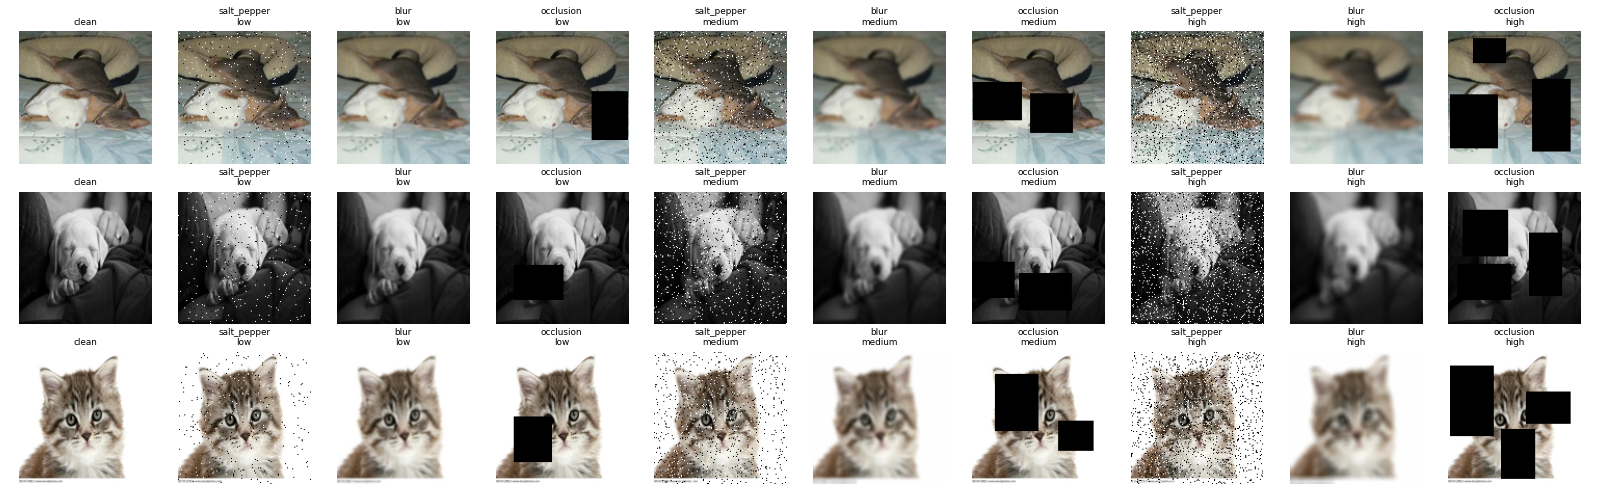
\includegraphics[width=\textwidth]{corruption_examples.png}
\caption{Test-manifest corruptions for three images (columns: clean, then salt-and-pepper, blur and occlusion at low/medium/high severity).}
\label{fig:corr}
\end{figure*}

\subsection{FS2K (Task 4)}
FS2K contains 1{,}058 official training pairs and 1{,}046 official test pairs with three sketch styles (style index 0/1/2 is shown as Style~1/2/3). 15\,\% of the training pairs (stratified by style, seed 42) form the validation set; the official test set is used only for the final evaluation. Photographs and sketches are resized to $128\times128$ with their pairing preserved. Paired augmentation applies the \emph{same} random horizontal flip and the \emph{same} random crop box (scale 0.8--1.0, resized back) to both images; a unit test checks that augmentation preserves alignment.

\section{Methods}
\subsection{Common training set-up}
Models are implemented in PyTorch. The restoration networks use AdamW \cite{loshchilov2019adamw} with a one-cycle learning-rate schedule \cite{smith2019onecycle}, gradient clipping at 5 and mixed precision on the GPU; GANs use Adam \cite{kingma2015adam} with $\beta=(0.5,0.999)$. Batch normalisation \cite{ioffe2015bn} is used in the convolutional blocks. The validation \emph{objective} used by every Optuna study is independent of any tuned loss weight: for restoration it is the mean validation $L_1+(1-\mathrm{SSIM})$ (lower is better); for the classifier $1-$macro-F1; for the GAN the validation $L_1+(1-\mathrm{SSIM})$ of generated against ground-truth sketches. SSIM is our own differentiable implementation (11$\times$11 Gaussian window, $\sigma=1.5$), unit-tested against scikit-image. PSNR is reported with a 50\,dB cap so that exact identity does not yield infinite values. All experiments are logged to MLflow (parameters, per-epoch curves, final checkpoints, sample images), and Optuna studies are stored in SQLite so that interrupted runs can resume.

\subsection{Task 1: universal denoising autoencoder}
\textbf{Architecture.} The encoder has four stride-2 convolutional stages ($128\to8$ pixels) whose channel count doubles from $c$ to $8c$, each stage being a $4\times4$ stride-2 convolution followed by a $3\times3$ convolution (batch norm, LeakyReLU). The $8\times8\times8c$ feature map is flattened and projected by a linear layer to a latent vector of dimension $d$ (dropout $p$), i.e.\ a compression of $49{,}152/d$ times; a linear layer re-expands it and four transposed-convolution stages and a final $3\times3$ convolution with a sigmoid reconstruct the $128\times128$ RGB image. There are no skip connections. The network is never told the corruption type. Fig.~\ref{fig:arch_ae} shows the layer dimensions of the selected configuration; this model has 2{,}401{,}347 learnable parameters (Table~\ref{tab:params}).

\textbf{Loss.} $\mathcal{L}=\alpha L_1(x,\hat{x})+(1-\alpha)(1-\mathrm{SSIM}(x,\hat{x}))$ with $x$ the clean target and $\hat{x}=D(E(\tilde{x}))$ the reconstruction of the corrupted input $\tilde{x}$.

\textbf{Optuna.} Learning rate, batch size, latent dimension $d$ (bottleneck), number of encoder channels $c$, dropout and $\alpha$ were searched (Table~\ref{tab:optuna_ae_universal_space}); each trial trains for a reduced budget on a subset of the training split, with median pruning.

\begin{figure*}[t]
\centering
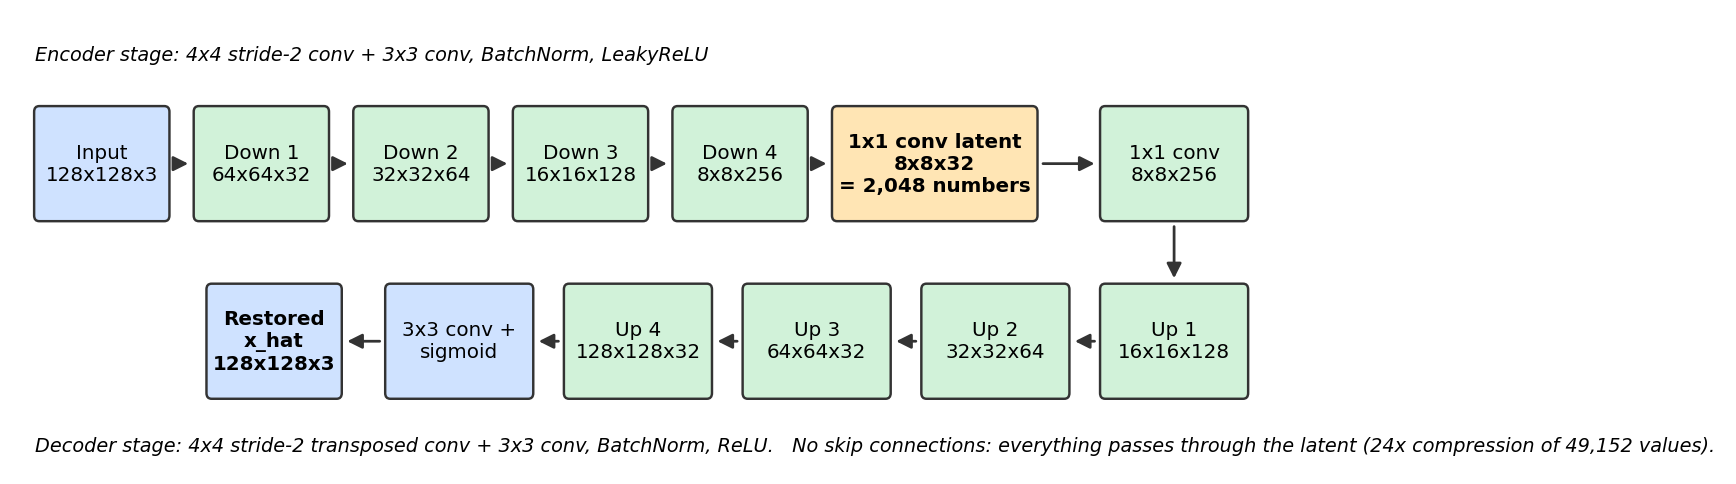
\includegraphics[width=0.95\textwidth]{arch_ae.png}
\caption{Architecture of the universal denoising autoencoder (Task~1) and of each Task~2 specialist for the selected configuration ($c=32$, spatial latent $8{\times}8{\times}32$): four stride-2 encoder stages, a $1{\times}1$-convolutional bottleneck of 2{,}048 numbers, four transposed-convolution decoder stages, and no skip connections.}
\label{fig:arch_ae}
\end{figure*}

\subsection{Task 2: classifier and hard-routed specialists}
\textbf{Classifier.} A plain CNN with $d_c$ conv blocks (two $3\times3$ convolutions each, channels $b,2b,\dots$ capped at $8b$, max pooling), global average pooling, dropout and a 4-way linear head, trained with multiclass cross-entropy on \emph{exactly class-balanced} batches (a custom batch sampler draws $B/4$ samples of every condition; labels come from the run-time pipeline).

\textbf{Specialists.} Three autoencoders of the Task~1 architecture are trained independently, each only on one corruption type (salt-and-pepper, blur, occlusion) with the same clean target and the $L_1$+SSIM loss. As allowed, one shared Optuna search selects a common architecture (learning rate, bottleneck, channels, batch size, $\alpha$): every trial trains the three specialists briefly and the objective is their mean validation objective. The selected architecture is the one of Fig.~\ref{fig:arch_ae}, so each specialist has 2{,}401{,}347 parameters and the classifier (five conv blocks, base 48 channels) 5{,}294{,}932 (Table~\ref{tab:params}).

\textbf{Inference.} With $r=\arg\max_k p_k$, the output is the identity for $r=$ clean (bypass, no expert is run) and $A_r(\tilde{x})$ otherwise. We evaluate two modes: \emph{oracle routing} (true label from the manifest) and \emph{predicted routing} (classifier decision). Fig.~\ref{fig:arch_routing}(a) summarises the pipeline.

\subsection{Task 3: jointly trained soft mixture-of-experts}
\label{sec:t3}
The gate is the Task~2 classifier; the experts are the three trained specialists; an identity branch handles clean inputs. With gate logits $G(\tilde{x})$ and temperature $\tau$, $w=\mathrm{softmax}(G(\tilde{x})/\tau)$ and $\hat{x}=w_0\tilde{x}+w_1A_{\mathrm{s\&p}}(\tilde{x})+w_2A_{\mathrm{blur}}(\tilde{x})+w_3A_{\mathrm{occ}}(\tilde{x})$, which is differentiable in both gate and experts. Training starts from the Task~2 weights (no random initialisation): first a warm-up stage with frozen experts trains only the gate, then all components are fine-tuned jointly with a smaller learning rate. The loss is
\begin{equation}
\mathcal{L}=\lambda_{1}L_{1}+\lambda_{2}(1-\mathrm{SSIM})+\lambda_{3}\,\mathrm{CE}\!\left(\tfrac{G(\tilde{x})}{\tau},y\right)+\lambda_{4}\sum_{k=0}^{3}\left(\bar{w}_k-\tfrac14\right)^2,
\end{equation}
with $\lambda_1=\alpha$, $\lambda_2=1-\alpha$, $\bar{w}_k$ the mean weight of branch $k$ over a class-balanced batch. The cross-entropy keeps the gate tied to the known run-time label (applied to the tempered logits so that it matches the routing weights actually used), and the squared-deviation balance term is a differentiable load-balancing regulariser in the spirit of \cite{shazeer2017moe,fedus2022switch}. Optuna tunes the joint learning rate, $\tau$, $\lambda_3$, $\lambda_4$ and $\alpha$; a trial is pruned when its intermediate objective is poor \emph{or} when routing collapses (a branch with mean validation weight below 0.02 or above 0.85). The complete pipeline (gate, experts, blending) is exported as one ONNX graph. Fig.~\ref{fig:arch_routing}(b) shows the architecture; the soft MoE has 12{,}498{,}973 parameters (classifier plus three specialists, Table~\ref{tab:params}).

\begin{figure*}[t]
\centering
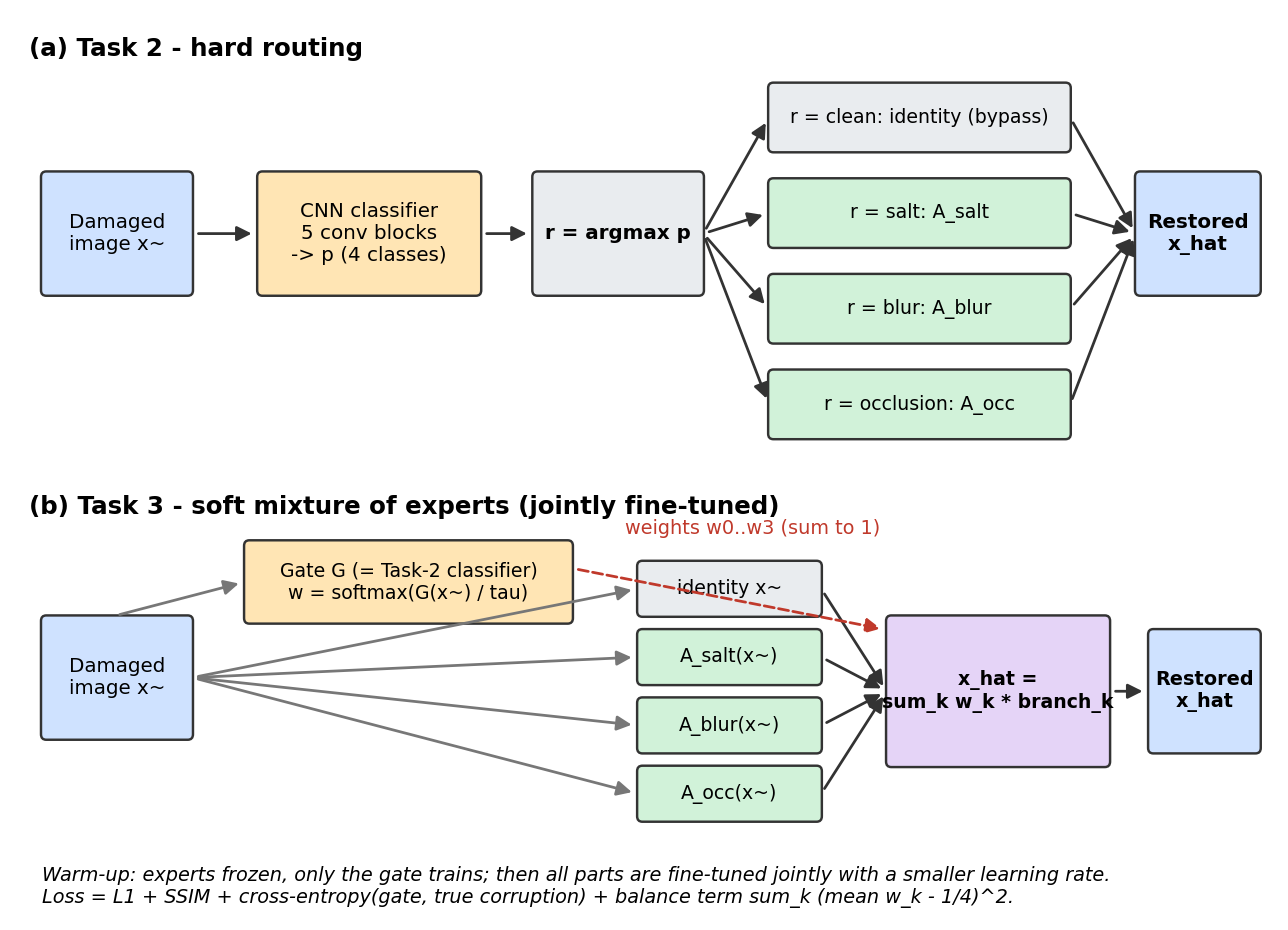
\includegraphics[width=0.9\textwidth]{arch_routing.png}
\caption{(a) Task~2 hard routing: the classifier probabilities are reduced by $\arg\max$ and select the identity bypass or one specialist. (b) Task~3 soft mixture of experts: the gate (initialised from the classifier) outputs temperature-softmax weights over the identity branch and the three experts, and the reconstruction is their weighted sum; gate and experts are trained jointly with the loss shown.}
\label{fig:arch_routing}
\end{figure*}

\subsection{Task 4: style-conditioned face-to-sketch cGAN}
\textbf{Generator.} A U-Net with seven stride-2 stages ($128\to1$) and a mirrored decoder with skip connections (dropout in the first three decoder stages). The style $s\in\{1,2,3\}$ is a \emph{learned embedding} of dimension $e$ that is (i) tiled over the image and concatenated to the input photograph and (ii) concatenated to the $1\times1$ bottleneck, so it influences both low-level and global features. The generator has 42{,}124{,}579 parameters (Table~\ref{tab:params}).

\textbf{Discriminator.} A PatchGAN that receives the concatenation of photograph, (real or generated) sketch and the tiled embedding of the same style from its own learned embedding table, and outputs a $14\times14$ map of real/fake logits (2{,}801{,}569 parameters). Fig.~\ref{fig:arch_gan} shows both networks.

\textbf{Losses.} $\mathcal{L}_D=\tfrac12[\mathrm{BCE}(D(x,y,s),1)+\mathrm{BCE}(D(x,G(x,s),s),0)]$ and $\mathcal{L}_G=\mathrm{BCE}(D(x,G(x,s),s),1)+\lambda_{L1}\lVert y-G(x,s)\rVert_1$. The discriminator real loss, discriminator fake loss, generator adversarial loss and generator $L_1$ loss are logged separately every epoch, together with validation $L_1$/PSNR/SSIM; the same six validation photographs are rendered at fixed intervals to monitor generator development. Optuna tunes the generator and discriminator learning rates, batch size, base channel count, dropout, style-embedding dimension and $\lambda_{L1}$ on shortened runs; the selected configuration is then retrained for the full schedule.

\begin{figure*}[t]
\centering
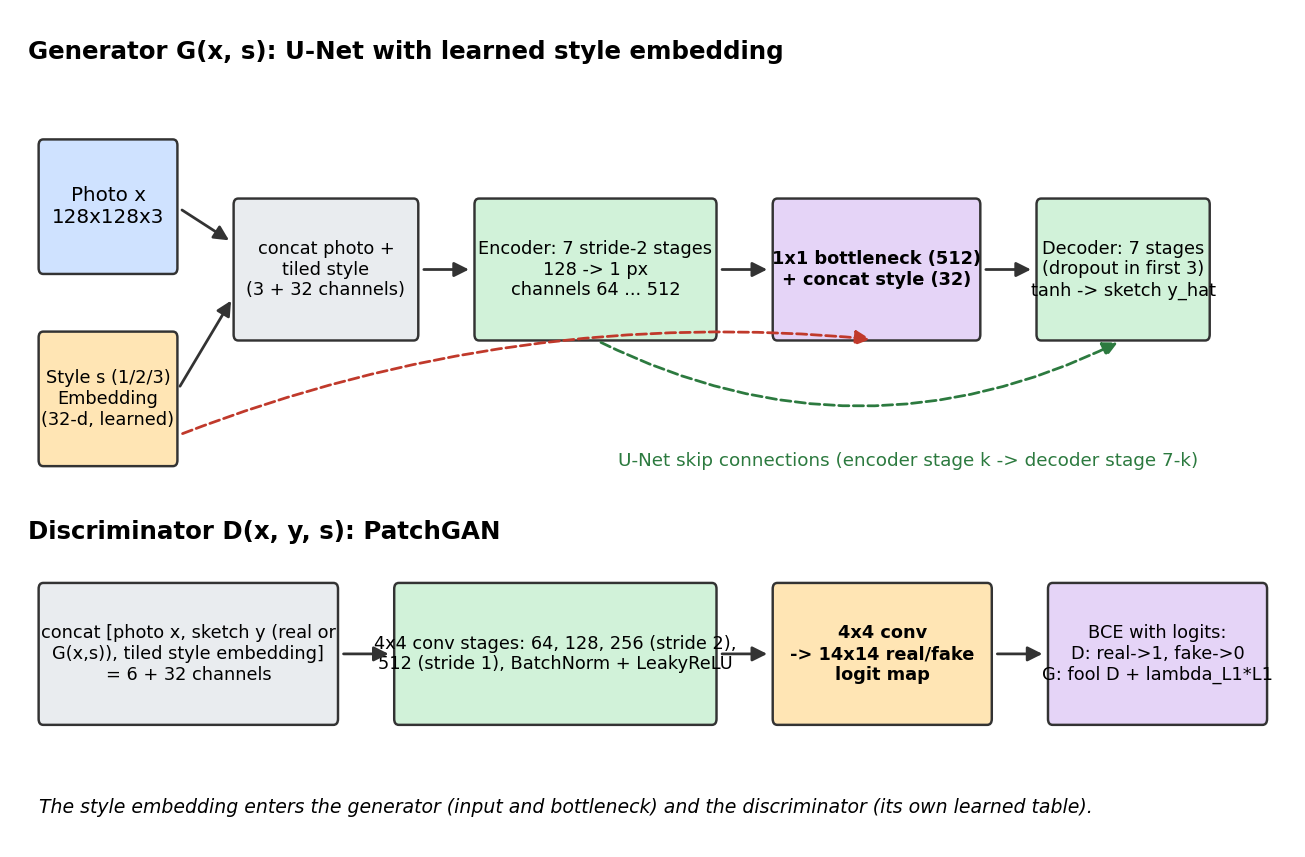
\includegraphics[width=0.92\textwidth]{arch_gan.png}
\caption{Task~4 architecture: U-Net generator with the learned style embedding injected at the input and at the bottleneck (top), and PatchGAN discriminator that receives photograph, sketch and the tiled style embedding (bottom).}
\label{fig:arch_gan}
\end{figure*}

\begin{table}[t]
\centering
\caption{Learnable parameters of the selected models (counted from the final configurations).}
\label{tab:params}
\footnotesize
\begin{tabular}{p{3.0cm}p{3.6cm}r}
\toprule
Model & Configuration & Parameters \\
\midrule
Task 1 universal autoencoder & $c=32$, spatial latent $8{\times}8{\times}32$ (2{,}048 numbers) & 2{,}401{,}347 \\
Task 2 specialist autoencoder (each of 3) & $c=32$, spatial latent $8{\times}8{\times}32$ & 2{,}401{,}347 \\
Task 2 classifier (= Task 3 gate) & 5 conv blocks, base 48 channels & 5{,}294{,}932 \\
Task 3 soft MoE (gate + 3 experts) & classifier + 3 specialists, $\tau$ fixed & 12{,}498{,}973 \\
Task 4 generator (U-Net) & base 64 channels, style embedding 32 & 42{,}124{,}579 \\
Task 4 discriminator (PatchGAN) & base 64 channels, style embedding 32 & 2{,}801{,}569 \\
\bottomrule
\end{tabular}
\end{table}


\section{Application and Deployment}
\label{sec:app}
\textbf{Design.} The interface was designed first in Google Stitch (Fig.~\ref{fig:stitch}); the React/Tailwind frontend follows its palette (indigo/cyan/teal on dark), fonts (Space Grotesk, Geist) and layout (left navigation with four workspaces, control card, image-panel grid, statistics card).

\begin{figure*}[t]
\centering
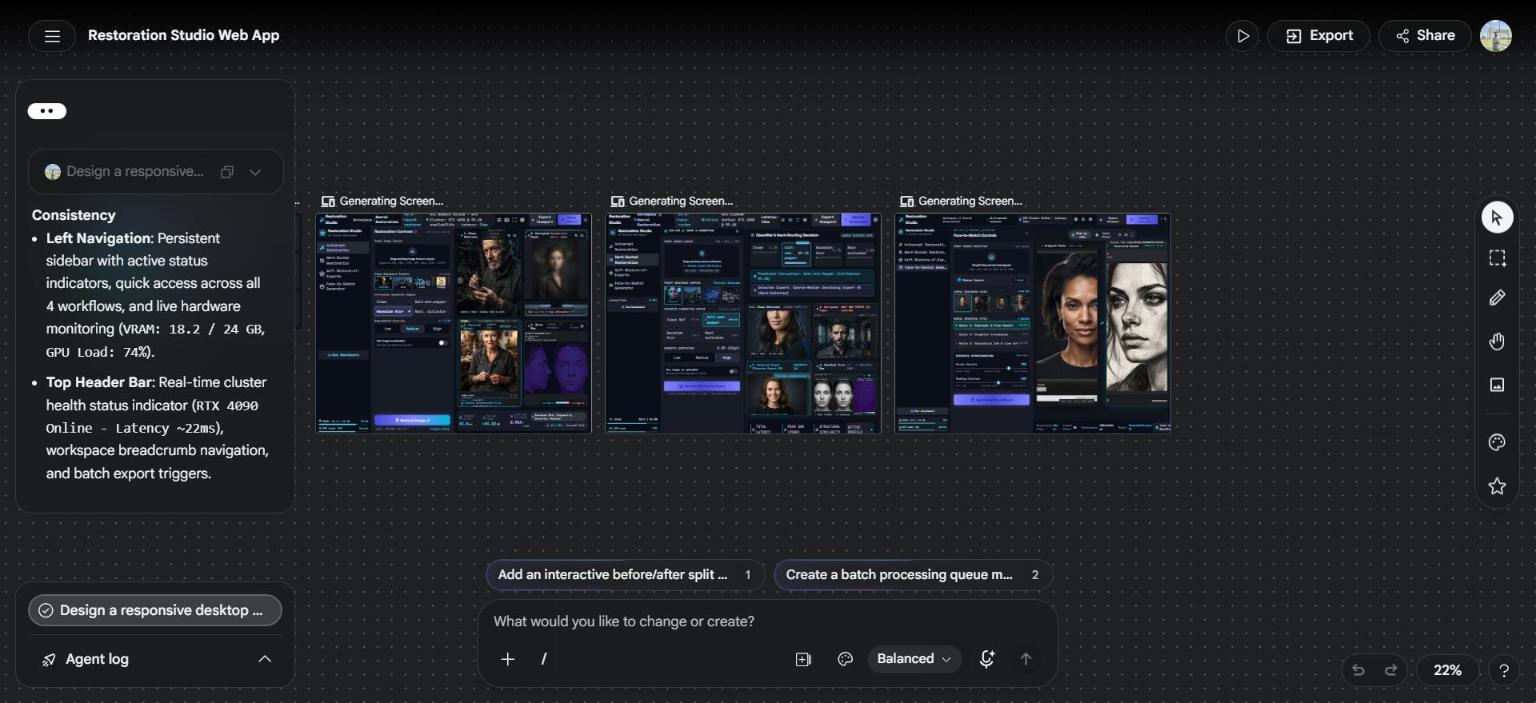
\includegraphics[width=0.95\textwidth]{stitch_canvas_overview.jpg}
\caption{Original Google Stitch design of ``Restoration Studio'' (design system and workspace screens) from which the React frontend was implemented.}
\label{fig:stitch}
\end{figure*}

\textbf{Architecture.} A React + Tailwind single-page application (served by nginx in its own container) calls a FastAPI backend (second container). The backend validates uploads (size limit, real-image check, allowed formats), resizes to $128\times128$, optionally applies the selected corruption with the \emph{same} algorithms as training (a NumPy/OpenCV re-implementation that is unit-tested against the training code), runs the ONNX models with ONNX Runtime, and returns base64 PNGs, routing information and timings. Endpoints: \texttt{GET /api/health}, \texttt{GET /api/samples}, \texttt{POST /api/universal}, \texttt{/api/hard-route}, \texttt{/api/soft-moe} and \texttt{/api/sketch}. The four workspaces are: \emph{Universal Restoration} (input, restored output, error map, corruption settings, inference time), \emph{Hard-Routed Restoration} (four classifier probabilities, predicted corruption, selected expert, output, timing), \emph{Soft Mixture-of-Experts} (four routing weights with the strongest contributors highlighted, output, timing) and \emph{Face-to-Sketch Generator} (upload or webcam, Style~1/2/3, side-by-side photo/sketch, download). \texttt{docker compose up --build} starts both containers; the ONNX models are mounted from \texttt{./models}. Screenshots of the running application are in Section~\ref{sec:appshots}.

\section{Experiments and Results}
All numbers in this section are measured on the \emph{official test sets} (Pet test: 3{,}669 images $\times$ 10 conditions $=$ 36{,}690 manifest entries; FS2K test: 1{,}046 pairs) with the final selected models, and are produced by the evaluation scripts in the repository; the tables are generated directly from the result files (\texttt{results/}). Hyper-parameter searches used reduced budgets (Section~\ref{sec:limits}); the final models were retrained for the full schedule with the selected configuration. Training ran on a Colab T4 GPU. ``Input'' denotes the unrestored corrupted image compared with the clean target (a baseline for how much the model improves the image). PSNR is in dB.

\subsection{Task 1: Universal Autoencoder}
\label{sec:t1}
\textbf{Optuna.} 24 trials (15 completed, 9 pruned by the median pruner) searched learning rate, batch size, bottleneck type and size, encoder channels, dropout and $\alpha$ (Tables~\ref{tab:optuna_ae_universal_space} and \ref{tab:optuna_ae_universal_best}). The first search, which only contained a \emph{dense} (fully-connected) latent vector of 128--1024 numbers, converged to a best validation objective of 0.735 and produced very blurry reconstructions (test: 18.37\,dB, SSIM 0.454; Fig.~\ref{fig:t1dense}). Inspecting those outputs showed that a global fully-connected code discards spatial layout, so a second search added a \emph{spatial} bottleneck (a $1\times1$-convolutional latent map of $64\cdot c_{\mathrm{lat}}$ numbers that keeps the $8\times8$ layout; still no skip connections). Optuna selected the spatial type (best objective 0.506) with $c_{\mathrm{lat}}=32$, i.e.\ a 2{,}048-number latent, a $24\times$ compression of the 49{,}152 input values, and $\alpha=0.554$ (the initial guess 0.8 was not optimal). The dense baseline is kept in the repository (\texttt{results/dense\_baseline}) and used as an ablation.

\begin{table}[t]
\centering
\caption{Optuna search space: Task 1 universal autoencoder.}
\label{tab:optuna_ae_universal_space}
\footnotesize
\begin{tabular}{ll}
\toprule
Hyper-parameter & Distribution \\
\midrule
lr & loguniform[1e-4, 3e-3] \\
batch\_size & categorical{32, 64, 128} \\
latent\_type & categorical{dense, spatial} \\
latent\_dim (dense) & categorical{128, 256, 512, 1024} \\
latent\_ch (spatial; dim = 64 x latent\_ch) & categorical{4, 8, 16, 32} \\
base\_ch & categorical{16, 32, 48, 64} \\
dropout & uniform[0.0, 0.3] \\
alpha & uniform[0.5, 0.95] \\
\bottomrule
\end{tabular}
\end{table}

\begin{table}[t]
\centering
\caption{Optuna result: Task 1 universal autoencoder.}
\label{tab:optuna_ae_universal_best}
\footnotesize
\begin{tabular}{ll}
\toprule
Item & Value \\
\midrule
lr & 0.00090 \\
batch\_size & 32 \\
latent\_type & spatial \\
base\_ch & 32 \\
alpha & 0.55424 \\
latent\_ch & 32 \\
dropout & 0.07002 \\
trials (complete / pruned / total) & 15 / 9 / 24 \\
best trial \#, objective & 23, 0.5062 \\
\bottomrule
\end{tabular}
\end{table}


\begin{figure*}[t]
\centering
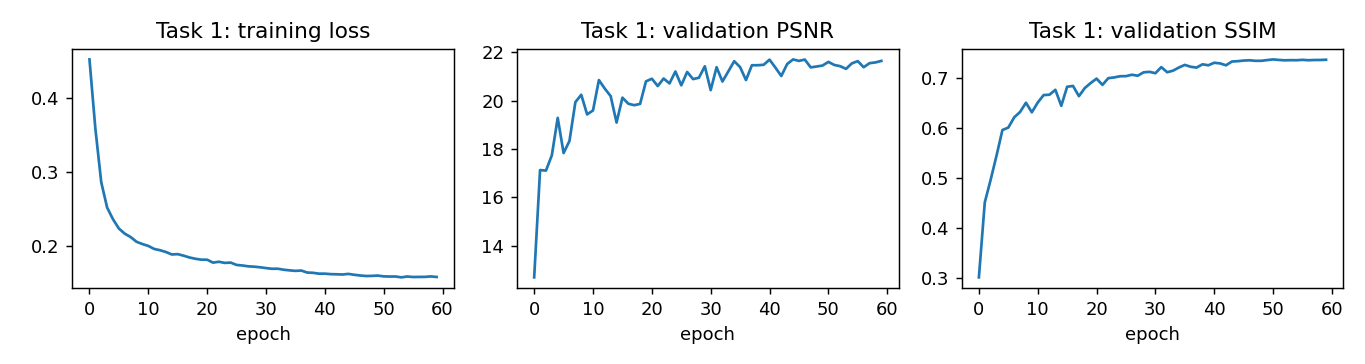
\includegraphics[width=\textwidth]{curves_task1.png}
\caption{Task 1 final training: training loss and validation PSNR/SSIM per epoch (from MLflow).}
\label{fig:curves1}
\end{figure*}

\begin{table}[t]
\centering
\caption{Task 1 test results (PSNR in dB). Input = unrestored corrupted image.}
\label{tab:t1_test}
\footnotesize
\begin{tabular}{lrrrrr}
\toprule
Condition & PSNR in & PSNR out & SSIM in & SSIM out & n \\
\midrule
clean & 50.00 & 21.96 & 1.000 & 0.761 & 3669 \\
salt\_pepper / low & 20.14 & 21.95 & 0.603 & 0.758 & 3669 \\
salt\_pepper / medium & 15.87 & 21.93 & 0.339 & 0.751 & 3669 \\
salt\_pepper / high & 13.14 & 21.84 & 0.204 & 0.737 & 3669 \\
blur / low & 32.34 & 22.06 & 0.944 & 0.760 & 3669 \\
blur / medium & 26.77 & 22.04 & 0.806 & 0.753 & 3669 \\
blur / high & 24.35 & 21.61 & 0.692 & 0.711 & 3669 \\
occlusion / low & 16.67 & 20.71 & 0.861 & 0.718 & 3669 \\
occlusion / medium & 13.32 & 19.74 & 0.727 & 0.675 & 3669 \\
occlusion / high & 10.73 & 18.49 & 0.537 & 0.611 & 3669 \\
\textbf{overall} & 22.33 & 21.23 & 0.671 & 0.723 & 36690 \\
\bottomrule
\end{tabular}
\end{table}


\textbf{Results.} Over all test conditions the universal autoencoder reaches 21.23\,dB / 0.723 SSIM against 22.33\,dB / 0.671 for the unrestored input (Table~\ref{tab:t1_test}). Its behaviour depends strongly on the damage: for salt-and-pepper noise it improves the image substantially (16.4$\to$21.9\,dB, SSIM 0.38$\to$0.75) and the gain grows with severity (13.1$\to$21.8\,dB at $p=0.15$); for occlusion it recovers PSNR (13.6$\to$19.7\,dB; 10.7$\to$18.5\,dB for 35\,\% coverage) but SSIM drops slightly (0.709$\to$0.668); for blur and for \emph{clean} inputs it is \emph{worse} than the input (e.g.\ blur/low 32.3$\to$22.1\,dB, clean 50$\to$22.0\,dB). This is the cost of the genuine bottleneck: every pixel must be regenerated from a $24\times$ compressed code, so the output quality saturates at about 22\,dB irrespective of the input quality (the output PSNR varies by only $\approx$0.1\,dB across the three salt-and-pepper severities), whereas inputs with mild damage are already better than that. This observation motivates the identity branch used in Tasks 2 and 3. Fig.~\ref{fig:t1ex} shows twelve representative test examples (clean, three severities of each corruption, and two random cases) with the absolute error map. Compared with the dense baseline (Fig.~\ref{fig:t1dense}) the spatial latent retains object shape, edges and colour, confirming the benefit of the convolutional prior.

\begin{figure*}[t]
\centering
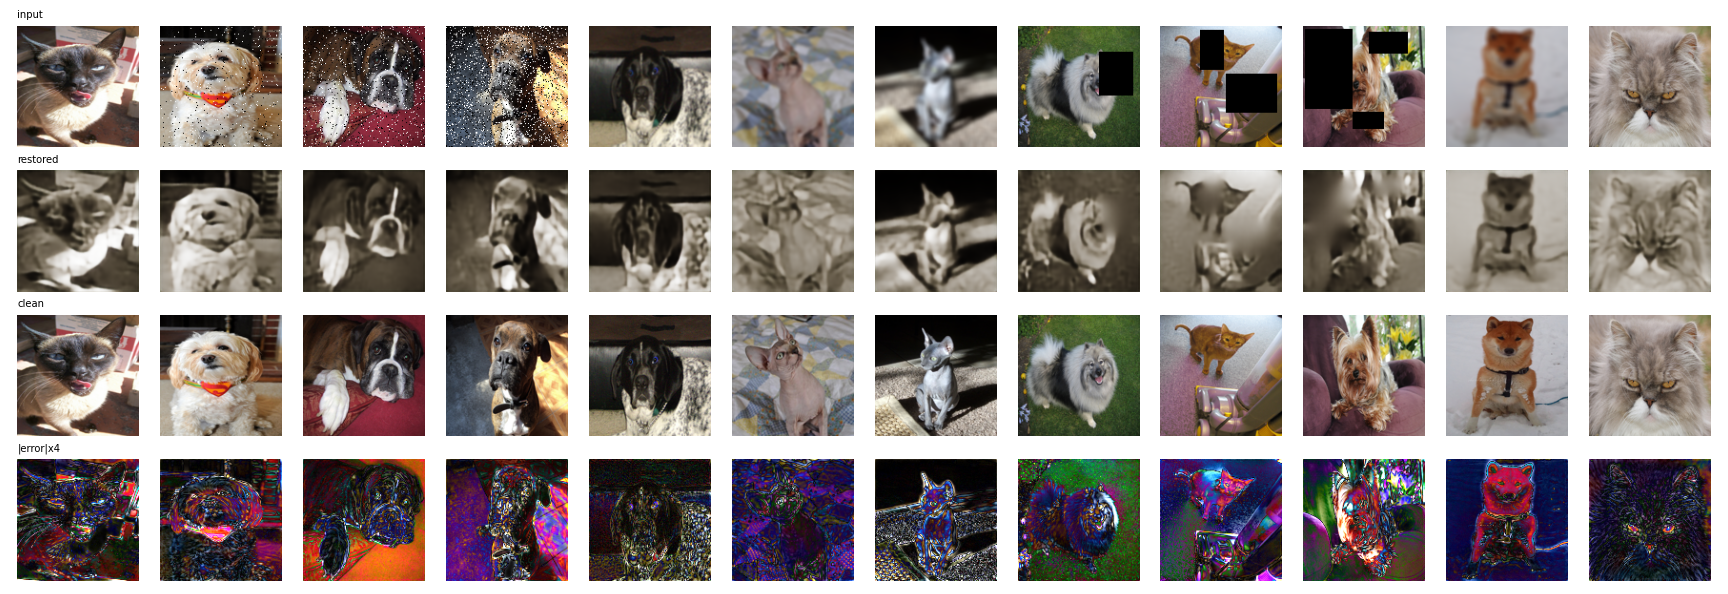
\includegraphics[width=\textwidth]{t1_examples.png}
\caption{Task 1, twelve representative test examples (rows: corrupted input, restored output, clean target, $4\times$ absolute error). Columns follow the manifest: clean, salt-and-pepper (low/medium/high), blur (low/medium/high), occlusion (low/medium/high) and two random cases.}
\label{fig:t1ex}
\end{figure*}

\begin{figure}[t]
\centering
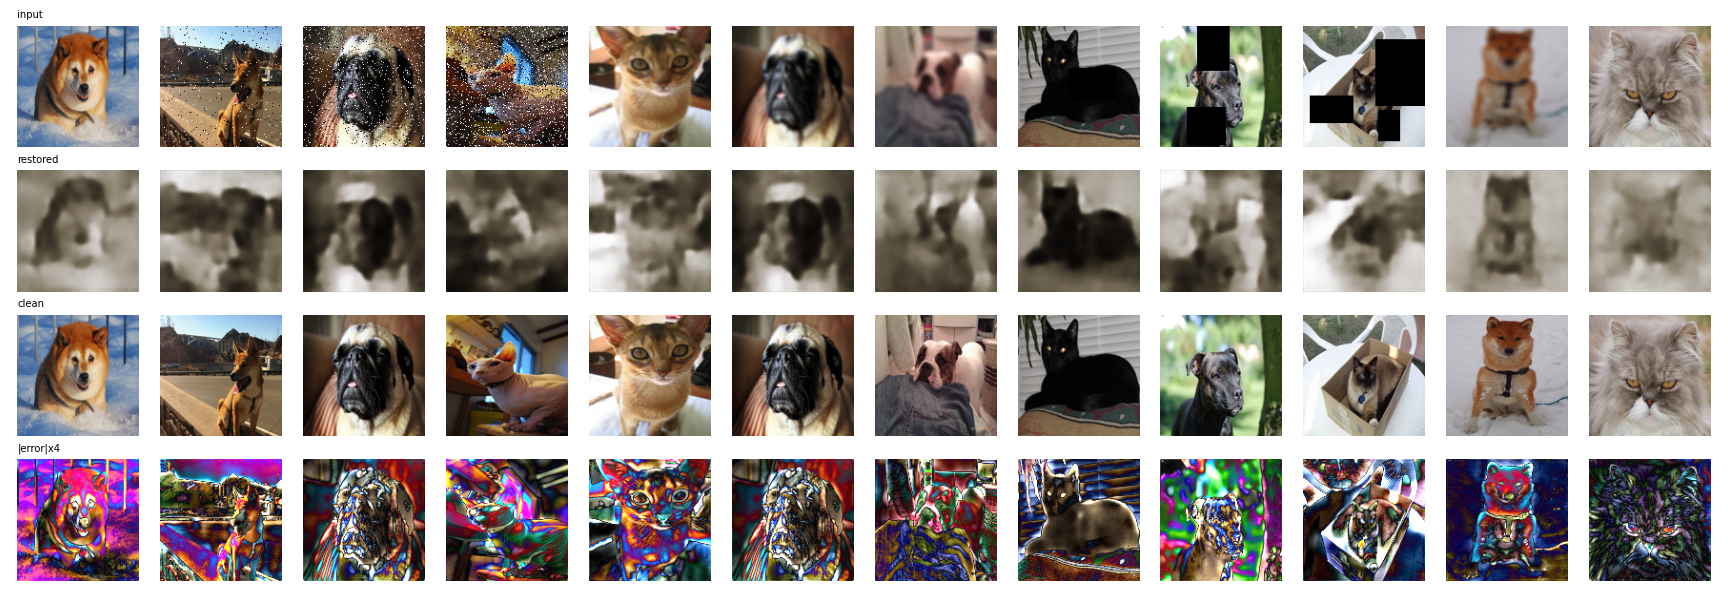
\includegraphics[width=\columnwidth]{t1_dense_examples.png}
\caption{Ablation: the same test examples reconstructed by the dense-bottleneck autoencoder of the first search (18.37\,dB, SSIM 0.454): only coarse colour blobs survive.}
\label{fig:t1dense}
\end{figure}

\textbf{Failure cases.} Fig.~\ref{fig:t1fail} shows the worst (lowest-SSIM) test example for each type. (i) \emph{Clean} (11.8\,dB): a pale cat on a pure black background; the network cannot reproduce the sharp black/white transition and leaks a brown halo into the background, an artefact of the bottleneck. (ii) \emph{Salt-and-pepper, $p=0.15$} (15.8\,dB) and (iii) \emph{blur, $\sigma=2.5$} (16.0\,dB): the same highly textured meadow image is the worst case for both, because its high-frequency detail is neither present in the blurred input nor representable in the latent. (iv) \emph{Occlusion, 35\,\%} (10.4\,dB, SSIM 0.25): the black masks hide most of the cat's body against a black background; the model fills the hole with a smooth grey region (no semantic inpainting), and this mismatch dominates the error map.

\begin{figure}[t]
\centering
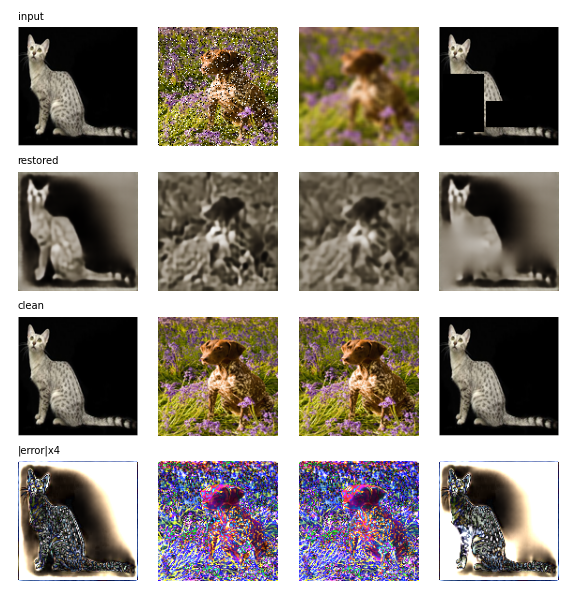
\includegraphics[width=\columnwidth]{t1_failures.png}
\caption{Task 1 failure cases (worst clean, salt-and-pepper, blur and occlusion test examples).}
\label{fig:t1fail}
\end{figure}

\subsection{Task 2: Classifier and Hard-Routed Specialists}
\textbf{Optuna and training.} The classifier search (20 trials, 7 completed, 13 pruned; Tables~\ref{tab:optuna_cls_space}, \ref{tab:optuna_cls_best}) chose five conv blocks with 48 base channels, dropout 0.47 and a small weight decay. The shared specialist search (14 trials, 8 completed; Tables~\ref{tab:optuna_ae_specialist_space}, \ref{tab:optuna_ae_specialist_best}) again preferred the spatial bottleneck ($c_{\mathrm{lat}}=32$, $\alpha=0.688$). The three specialists were then trained independently, each only on its own corruption.

\begin{table}[t]
\centering
\caption{Optuna search space: Task 2 corruption classifier.}
\label{tab:optuna_cls_space}
\footnotesize
\begin{tabular}{ll}
\toprule
Hyper-parameter & Distribution \\
\midrule
lr & loguniform[1e-4, 3e-3] \\
batch\_size & categorical{32, 64, 128} \\
base\_ch & categorical{16, 32, 48} \\
depth & categorical{3, 4, 5} \\
dropout & uniform[0.0, 0.5] \\
weight\_decay & loguniform[1e-6, 1e-2] \\
\bottomrule
\end{tabular}
\end{table}

\begin{table}[t]
\centering
\caption{Optuna result: Task 2 corruption classifier.}
\label{tab:optuna_cls_best}
\footnotesize
\begin{tabular}{ll}
\toprule
Item & Value \\
\midrule
lr & 0.00050 \\
batch\_size & 32 \\
base\_ch & 48 \\
depth & 5 \\
dropout & 0.46691 \\
weight\_decay & 0.00002 \\
trials (complete / pruned / total) & 7 / 13 / 20 \\
best trial \#, objective & 11, 0.0128 \\
\bottomrule
\end{tabular}
\end{table}

\begin{table}[t]
\centering
\caption{Optuna search space: Task 2 specialist autoencoders (shared search).}
\label{tab:optuna_ae_specialist_space}
\footnotesize
\begin{tabular}{ll}
\toprule
Hyper-parameter & Distribution \\
\midrule
lr & loguniform[1e-4, 3e-3] \\
batch\_size & categorical{32, 64, 128} \\
latent\_type & categorical{dense, spatial} \\
latent\_dim (dense) & categorical{128, 256, 512, 1024} \\
latent\_ch (spatial; dim = 64 x latent\_ch) & categorical{4, 8, 16, 32} \\
base\_ch & categorical{16, 32, 48, 64} \\
alpha & uniform[0.5, 0.95] \\
(fixed) dropout & 0.1 \\
\bottomrule
\end{tabular}
\end{table}

\begin{table}[t]
\centering
\caption{Optuna result: Task 2 specialist autoencoders (shared search).}
\label{tab:optuna_ae_specialist_best}
\footnotesize
\begin{tabular}{ll}
\toprule
Item & Value \\
\midrule
lr & 0.00156 \\
batch\_size & 32 \\
latent\_type & spatial \\
base\_ch & 32 \\
alpha & 0.68783 \\
latent\_ch & 32 \\
trials (complete / pruned / total) & 8 / 6 / 14 \\
best trial \#, objective & 8, 0.5229 \\
\bottomrule
\end{tabular}
\end{table}


\begin{figure*}[t]
\centering
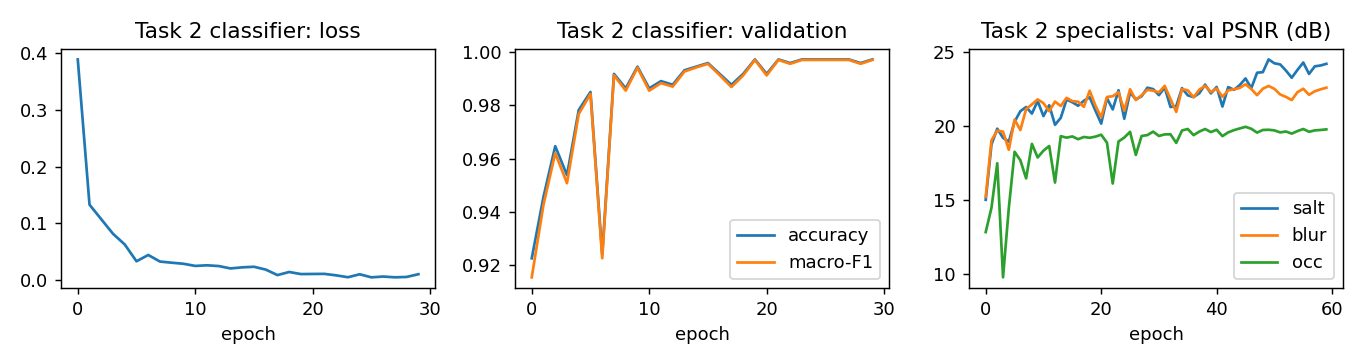
\includegraphics[width=\textwidth]{curves_task2.png}
\caption{Task 2: classifier loss and validation accuracy/F1, and validation PSNR of the three specialists.}
\label{fig:curves2}
\end{figure*}

\begin{table}[t]
\centering
\caption{Task 2 classifier, per-class test metrics.}
\label{tab:t2_cls}
\footnotesize
\begin{tabular}{lrrrr}
\toprule
Class & Precision & Recall & F1 & Support \\
\midrule
clean & 0.969 & 0.994 & 0.982 & 3669 \\
salt\_pepper & 1.000 & 1.000 & 1.000 & 11007 \\
blur & 0.998 & 1.000 & 0.999 & 11007 \\
occlusion & 1.000 & 0.990 & 0.995 & 11007 \\
\textbf{macro avg} & 0.992 & 0.996 & 0.994 &  \\
\textbf{accuracy} &  &  & 0.996 &  \\
\bottomrule
\end{tabular}
\end{table}


\textbf{Classifier.} On the 36{,}690 test entries the classifier reaches accuracy 0.9963, macro-precision 0.9919, macro-recall 0.9959 and macro-F1 0.9939 (Table~\ref{tab:t2_cls}); the normalised confusion matrix is in Fig.~\ref{fig:t2cm}. Salt-and-pepper noise is recognised perfectly at all three severities, blur almost perfectly (recall 0.9997; 0.9992 at the weakest setting $k=3,\sigma=0.7$). The only noticeable confusion involves the clean class: 1.0\,\% of occluded images are called clean, almost all of them the weakest occlusion (recall 0.9695 for the single 10\,\% rectangle, which hides little), and 0.5\,\% of clean images are called blur; the lowest precision (0.969) belongs to the clean class because it receives these errors, and it has a smaller support (3{,}669 vs.\ 11{,}007).

\begin{figure}[t]
\centering
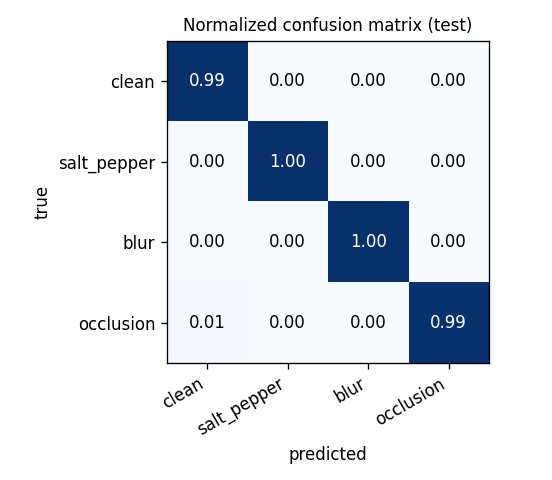
\includegraphics[width=0.8\columnwidth]{t2_confusion.png}
\caption{Task 2: normalised four-class confusion matrix on the test manifest.}
\label{fig:t2cm}
\end{figure}

\begin{table}[t]
\centering
\caption{Task 2 test restoration with oracle vs.\ predicted routing.}
\label{tab:t2_rest}
\footnotesize
\begin{tabular}{lrrrr}
\toprule
Condition & PSNR oracle & SSIM oracle & PSNR pred. & SSIM pred. \\
\midrule
clean & 50.00 & 1.000 & 49.83 & 0.999 \\
salt\_pepper / low & 23.82 & 0.769 & 23.82 & 0.769 \\
salt\_pepper / medium & 23.80 & 0.767 & 23.80 & 0.767 \\
salt\_pepper / high & 23.75 & 0.763 & 23.75 & 0.763 \\
blur / low & 22.28 & 0.761 & 22.29 & 0.761 \\
blur / medium & 22.35 & 0.759 & 22.35 & 0.759 \\
blur / high & 22.03 & 0.729 & 22.03 & 0.729 \\
occlusion / low & 20.94 & 0.701 & 21.02 & 0.707 \\
occlusion / medium & 20.07 & 0.665 & 20.07 & 0.665 \\
occlusion / high & 18.90 & 0.608 & 18.90 & 0.608 \\
\textbf{overall} & 24.79 & 0.752 & 24.79 & 0.753 \\
\bottomrule
\end{tabular}
\end{table}


\textbf{Restoration with oracle and predicted routing.} Table~\ref{tab:t2_rest} gives the two modes. Overall the system reaches 24.79\,dB in both modes (SSIM 0.752 oracle, 0.753 predicted), against 22.33\,dB / 0.671 for the input and 21.23\,dB / 0.723 for the universal autoencoder of Task~1; since the classifier is almost perfect, predicted routing loses nothing measurable relative to oracle routing. Part of the gain comes simply from the identity bypass: clean images are returned exactly (49.8\,dB with the 50\,dB cap) while Task~1 damaged them. On \emph{corrupted} images only, the specialists beat the universal model by 1.9\,dB (salt-and-pepper: 23.79 vs.\ 21.90), 0.3\,dB (blur: 22.22 vs.\ 21.91) and 0.3\,dB (occlusion: 19.97 vs.\ 19.65): specialisation helps most when the corruption has a simple, learnable inverse (noise) and little when the missing information cannot be recovered (blur, occlusion). As in Task~1, the blur specialist is below the input PSNR (22.2 vs.\ 27.8\,dB).

\textbf{Routing failures.} 137 of 36{,}690 test entries (0.37\,\%) were misrouted. The damaging cases are not those where a corrupted image is sent to the wrong expert but those where a \emph{clean} image is classified as corrupted: the selected expert then regenerates the image from its latent code and destroys its fidelity. Fig.~\ref{fig:t2fail} shows the four worst: clean images routed to the blur expert (50\,dB $\to$ 10.8, 11.9 and 12.0\,dB) or to the occlusion expert (50 $\to$ 13.6\,dB). Misrouted images lost on average 2.3\,dB relative to oracle routing; this is the weakness of hard routing that Task~3 addresses.

\begin{figure}[t]
\centering
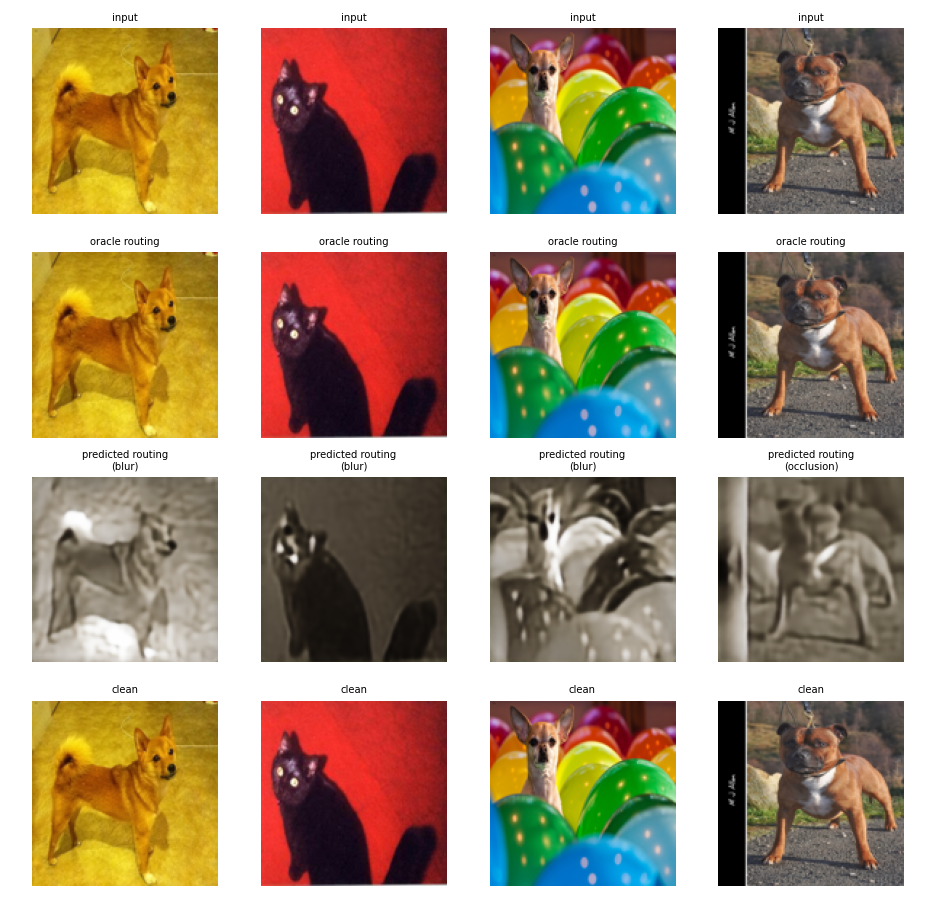
\includegraphics[width=\columnwidth]{t2_routing_failures.png}
\caption{Task 2 routing failures: clean test images sent to a restoration expert by the classifier (rows: input, oracle routing = identity, predicted routing, clean).}
\label{fig:t2fail}
\end{figure}

\subsection{Task 3: Soft Mixture-of-Experts}
\textbf{Optuna.} The 15-trial study (Tables~\ref{tab:optuna_moe_space}, \ref{tab:optuna_moe_best}) tuned the joint learning rate, temperature, $\lambda_{CE}$, $\lambda_{bal}$ and $\alpha$; trials with a collapsed or dominating branch would have been pruned, but none of the 15 trials collapsed. The selected configuration has $\tau=1.43$ (a slightly softened gate), $\lambda_{CE}=0.019$, $\lambda_{bal}=0.0074$ and $\alpha=0.725$. The training used 2 warm-up epochs (gate only, learning rate $3\times$ the joint one) followed by 18 joint epochs (Fig.~\ref{fig:curves3}); on the validation set the system started at 28.7\,dB (right after initialisation from Task~2, where the identity branch already helps clean images) and finished at 30.2\,dB.

\begin{table}[t]
\centering
\caption{Optuna search space: Task 3 joint fine-tuning.}
\label{tab:optuna_moe_space}
\footnotesize
\begin{tabular}{ll}
\toprule
Hyper-parameter & Distribution \\
\midrule
lr & loguniform[1e-5, 1e-3] \\
tau & loguniform[0.5, 2.0] \\
lambda\_ce & loguniform[0.01, 1.0] \\
lambda\_bal & loguniform[1e-3, 0.1] \\
alpha (L1 weight; SSIM weight = 1 - alpha) & uniform[0.5, 0.95] \\
\bottomrule
\end{tabular}
\end{table}

\begin{table}[t]
\centering
\caption{Optuna result: Task 3 joint fine-tuning.}
\label{tab:optuna_moe_best}
\footnotesize
\begin{tabular}{ll}
\toprule
Item & Value \\
\midrule
lr & 0.00063 \\
tau & 1.43144 \\
lambda\_ce & 0.01899 \\
lambda\_bal & 0.00742 \\
alpha & 0.72496 \\
trials (complete / pruned / total) & 15 / 0 / 15 \\
best trial \#, objective & 13, 0.2044 \\
\bottomrule
\end{tabular}
\end{table}


\begin{figure*}[t]
\centering
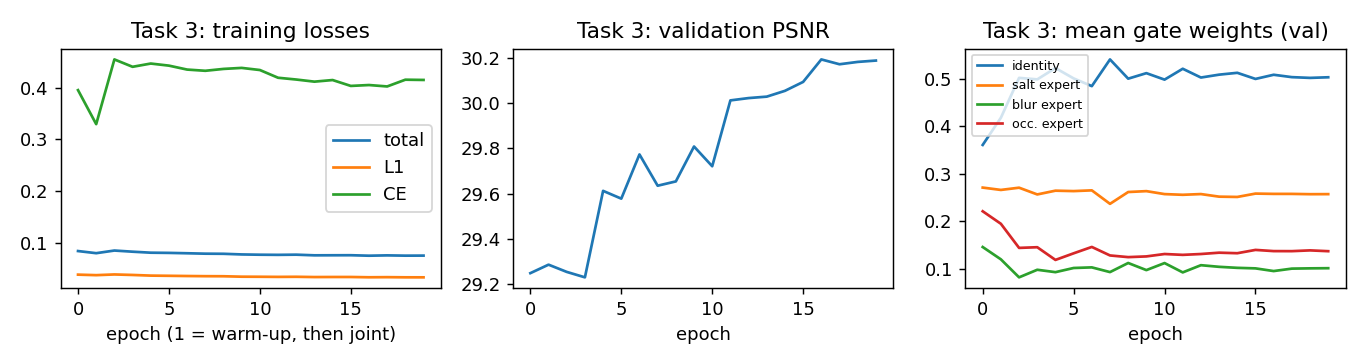
\includegraphics[width=\textwidth]{curves_task3.png}
\caption{Task 3 joint training: losses, validation PSNR and mean gate weights per branch.}
\label{fig:curves3}
\end{figure*}

\begin{table}[t]
\centering
\caption{Task 3 soft mixture-of-experts, test results (PSNR in dB).}
\label{tab:t3_test}
\footnotesize
\begin{tabular}{lrrrrr}
\toprule
Condition & PSNR in & PSNR out & SSIM in & SSIM out & n \\
\midrule
clean & 50.00 & 49.75 & 1.000 & 0.999 & 3669 \\
salt\_pepper / low & 20.14 & 24.57 & 0.603 & 0.804 & 3669 \\
salt\_pepper / medium & 15.87 & 23.90 & 0.339 & 0.777 & 3669 \\
salt\_pepper / high & 13.14 & 23.67 & 0.204 & 0.767 & 3669 \\
blur / low & 32.34 & 29.14 & 0.944 & 0.916 & 3669 \\
blur / medium & 26.77 & 25.65 & 0.806 & 0.814 & 3669 \\
blur / high & 24.35 & 24.27 & 0.692 & 0.751 & 3669 \\
occlusion / low & 16.67 & 22.09 & 0.861 & 0.866 & 3669 \\
occlusion / medium & 13.32 & 20.72 & 0.727 & 0.778 & 3669 \\
occlusion / high & 10.73 & 19.02 & 0.537 & 0.671 & 3669 \\
\textbf{overall} & 22.33 & 26.28 & 0.671 & 0.814 & 36690 \\
\bottomrule
\end{tabular}
\end{table}


\textbf{Restoration.} Table~\ref{tab:t3_test} reports 26.28\,dB / 0.814 SSIM overall, which is higher than hard routing (24.79\,dB / 0.753), the universal autoencoder (21.23\,dB / 0.723) and the input (22.33\,dB / 0.671); the corresponding model built on the dense bottleneck reached 24.40\,dB / 0.723. In particular, the soft blend closes the gap on blur: SSIM 0.827 is \emph{above} the input's 0.814 and PSNR is 26.4\,dB for blur (29.1\,dB at the lowest severity, versus 22.1 for the specialist alone), because the gate mixes the input with the expert's output instead of replacing it. Clean images stay at 49.8\,dB, and salt-and-pepper (24.0\,dB) and occlusion (20.6\,dB, SSIM 0.77) improve on Task~2 as well.

\begin{table}[t]
\centering
\caption{Mean gate weights per true condition (test).}
\label{tab:t3_weights}
\footnotesize
\begin{tabular}{lrrrr}
\toprule
Condition & identity & salt & blur & occ. \\
\midrule
clean & 0.995 & 0.000 & 0.003 & 0.003 \\
salt\_pepper & 0.073 & 0.925 & 0.001 & 0.001 \\
salt\_pepper/low & 0.153 & 0.841 & 0.003 & 0.003 \\
salt\_pepper/medium & 0.050 & 0.949 & 0.000 & 0.000 \\
salt\_pepper/high & 0.016 & 0.984 & 0.000 & 0.000 \\
blur & 0.579 & 0.000 & 0.420 & 0.000 \\
blur/low & 0.715 & 0.000 & 0.285 & 0.000 \\
blur/medium & 0.542 & 0.000 & 0.458 & 0.000 \\
blur/high & 0.481 & 0.000 & 0.519 & 0.000 \\
occlusion & 0.490 & 0.000 & 0.000 & 0.510 \\
occlusion/low & 0.582 & 0.000 & 0.000 & 0.418 \\
occlusion/medium & 0.472 & 0.000 & 0.000 & 0.528 \\
occlusion/high & 0.415 & 0.000 & 0.000 & 0.585 \\
\bottomrule
\end{tabular}
\end{table}


\textbf{Gate behaviour.} Table~\ref{tab:t3_weights} and Fig.~\ref{fig:t3heat} list the mean weights per true condition and severity. The gate has \emph{not} remained a pure classifier (argmax-routing accuracy 0.673, compared with 99.6\,\% for the initial classifier) because the reconstruction loss dominates the small classification weight selected by Optuna; instead it learned a severity-adaptive blending policy: clean $\to$ identity (0.99); salt-and-pepper $\to$ salt expert with weight rising from 0.84 (low) to 0.98 (high); blur $\to$ roughly equal identity and blur expert (0.71/0.28 at low, 0.48/0.52 at high); occlusion $\to$ identity plus occlusion expert (0.42 at low, 0.58 at high). Every expert is used only for its own corruption type (their weights for unrelated types are numerically zero), so no expert dominates unrelated inputs and none is inactive: the mean weights per branch are 0.442/0.278/0.127/0.154 (identity/salt/blur/occlusion), with the blur expert the least used, consistent with Task~2 where blur is the corruption that specialisation helps least. Fig.~\ref{fig:t3w} shows examples where one expert completely dominates (heavy salt-and-pepper noise: weight $\approx$1 on the salt expert) and examples where the weights are spread (lighter noise: about 0.65 identity, 0.25 salt expert). The load-balance term is not violated (no branch below 0.05), but note that ``balance'' is measured on a class-balanced batch: the identity branch still gets the largest average share.

\begin{table}[t]
\centering
\caption{Gate health on the test set.}
\label{tab:t3_health}
\footnotesize
\begin{tabular}{ll}
\toprule
Statistic & Value \\
\midrule
routing accuracy (argmax = true type) & 0.673 \\
mean weight per branch & 0.442, 0.278, 0.127, 0.154 \\
inactive branches (mean weight $<0.05$) & none \\
mean gate entropy (nats) & 0.451 \\
\bottomrule
\end{tabular}
\end{table}


\begin{figure}[t]
\centering
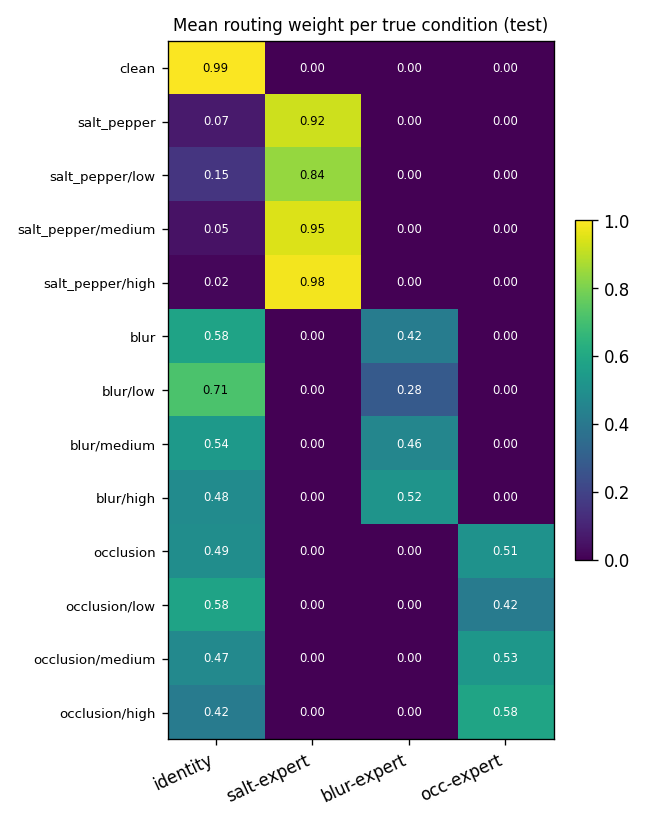
\includegraphics[width=\columnwidth]{t3_heatmap.png}
\caption{Task 3: mean routing weight per true corruption type and severity (test).}
\label{fig:t3heat}
\end{figure}

\begin{figure*}[t]
\centering
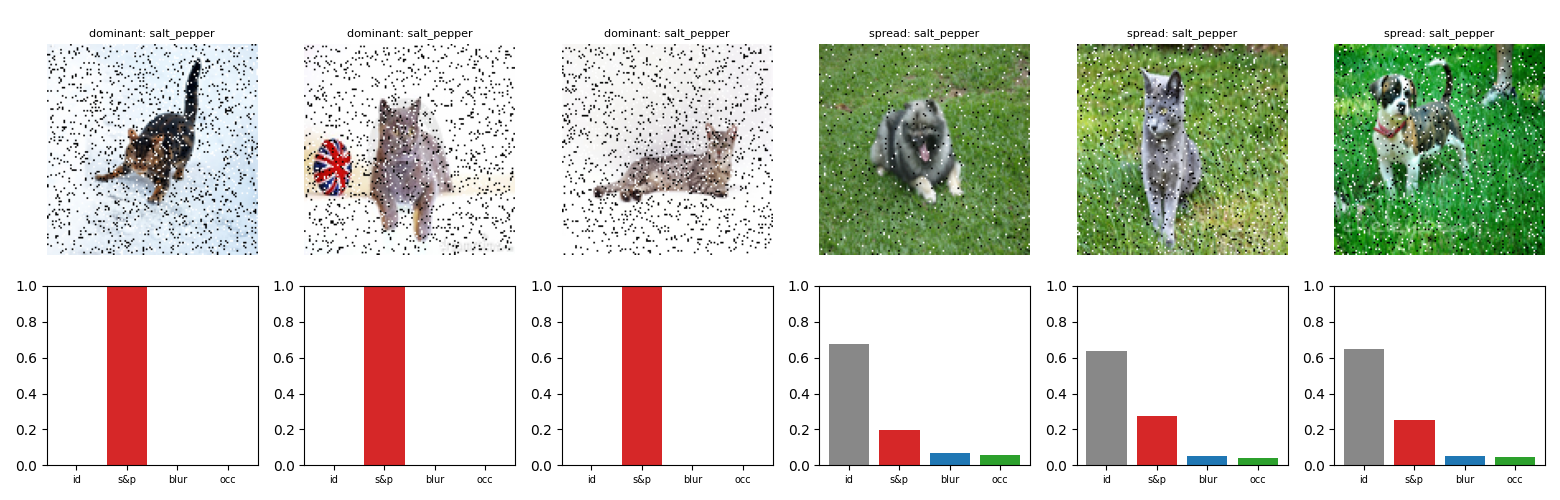
\includegraphics[width=\textwidth]{t3_weight_examples.png}
\caption{Task 3 routing weights for individual test images: one expert dominating (left three) and distributed weights (right three). Bars: identity, salt, blur, occlusion.}
\label{fig:t3w}
\end{figure*}

\begin{figure*}[t]
\centering
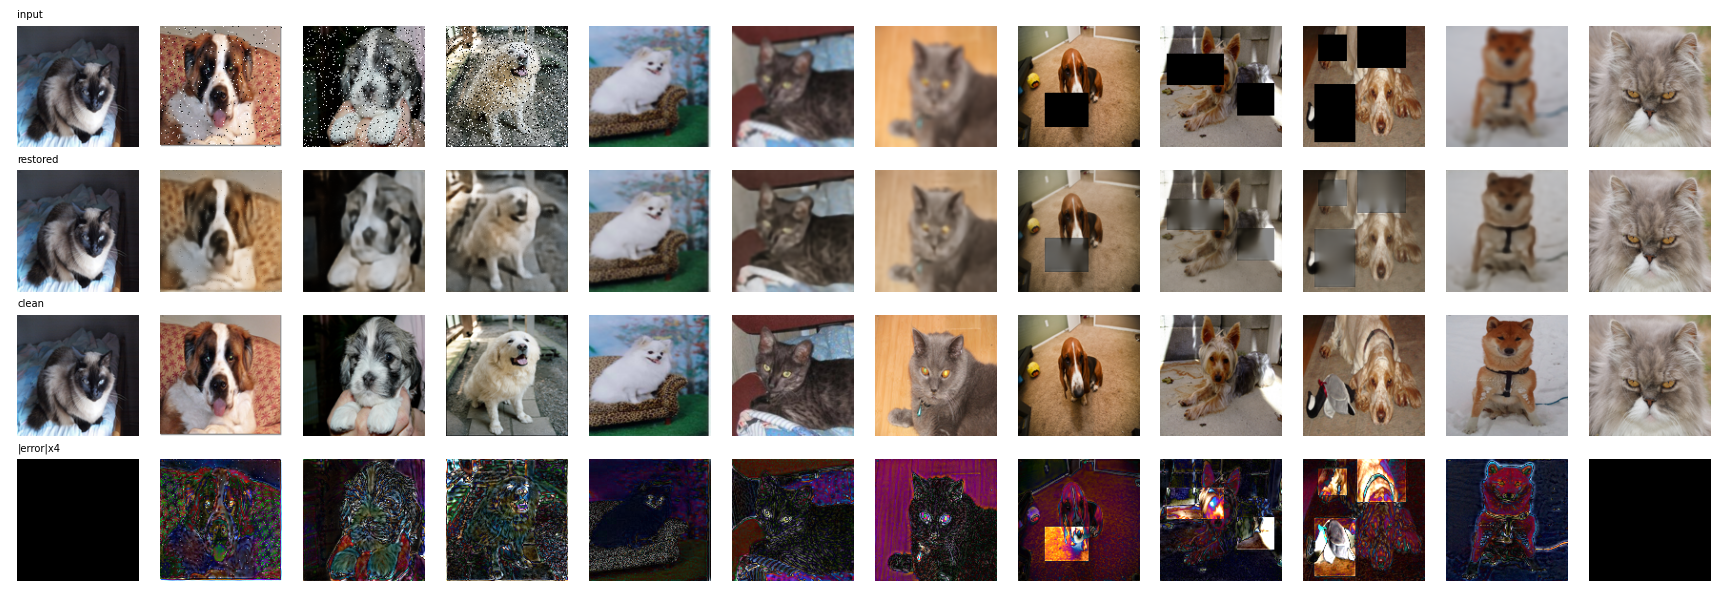
\includegraphics[width=\textwidth]{t3_examples.png}
\caption{Task 3 soft-MoE restoration: twelve representative test examples (input, restored, clean, $4\times$ error).}
\label{fig:t3ex}
\end{figure*}

\textbf{Failure cases.} The four worst cases (Fig.~\ref{fig:t3fail}) are: a clean image with large black areas for which the gate gives 0.53 weight to the occlusion expert (13.2\,dB): the gate confuses real dark regions with occlusion, the soft-MoE analogue of the hard-routing failure but milder because the identity still gets 0.47; a heavily textured salt-and-pepper image (17.5\,dB, weight 0.93 on the salt expert) whose texture cannot be regenerated; a strongly blurred image (18.1\,dB; weights 0.76 identity, 0.24 blur); and a large 35\,\% occlusion (10.8\,dB; 0.59 on the occlusion expert) in which the hole cannot be plausibly inpainted by an autoencoder.

\begin{figure}[t]
\centering
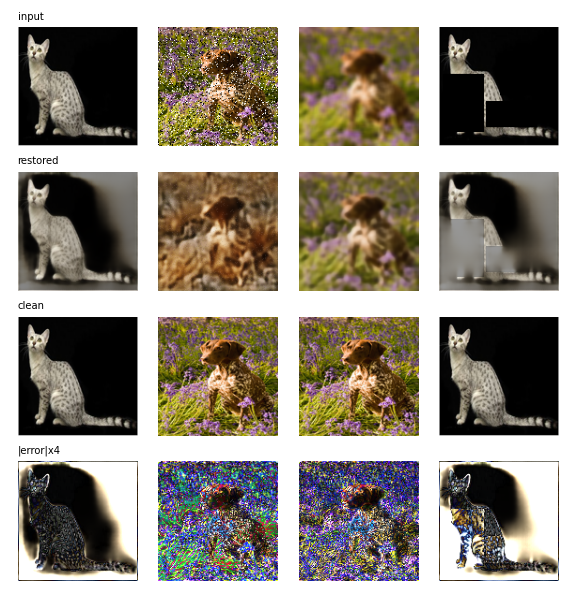
\includegraphics[width=\columnwidth]{t3_failures.png}
\caption{Task 3 failure cases (worst clean, salt-and-pepper, blur and occlusion).}
\label{fig:t3fail}
\end{figure}

\subsection{Task 4: Style-Conditioned Face-to-Sketch cGAN}
\textbf{Optuna and training.} The 12-trial study (6 completed, 6 pruned; Tables~\ref{tab:optuna_gan_space}, \ref{tab:optuna_gan_best}) used shortened runs of 10 epochs. It selected $g_{lr}=5.8\times10^{-4}$, $d_{lr}=6.6\times10^{-4}$, batch size 16, 64 base channels, dropout 0.47, a 32-dimensional style embedding and $\lambda_{L1}=272.5$ (near the upper edge of the searched range $[10,300]$, indicating that a strong pixel term helps on this small dataset). The selected configuration was retrained for the full 150 epochs; the best validation epoch is used. Fig.~\ref{fig:curves4} shows the separately logged discriminator real/fake losses, generator adversarial and $L_1$ losses and validation metrics; the discriminator stays near $0.35$--$0.45$ (neither side collapses) with an isolated instability near epoch 145. The training $L_1$ is higher than validation $L_1$ because training uses dropout and random paired crops. Fig.~\ref{fig:t4prog} shows the same validation photographs at epochs 1, 10, 50, 100 and 150: from an empty grey output at epoch 1 to recognisable faces at epoch 10 and sharp pencil-like strokes by epoch 50, after which improvements are subtle.

\begin{table}[t]
\centering
\caption{Optuna search space: Task 4 face-to-sketch cGAN.}
\label{tab:optuna_gan_space}
\footnotesize
\begin{tabular}{ll}
\toprule
Hyper-parameter & Distribution \\
\midrule
g\_lr & loguniform[5e-5, 1e-3] \\
d\_lr & loguniform[5e-5, 1e-3] \\
batch\_size & categorical{8, 16, 32} \\
base\_ch & categorical{32, 48, 64} \\
dropout & uniform[0.0, 0.5] \\
style\_dim & categorical{8, 16, 32, 64} \\
lambda\_l1 & loguniform[10, 300] \\
\bottomrule
\end{tabular}
\end{table}

\begin{table}[t]
\centering
\caption{Optuna result: Task 4 face-to-sketch cGAN.}
\label{tab:optuna_gan_best}
\footnotesize
\begin{tabular}{ll}
\toprule
Item & Value \\
\midrule
g\_lr & 0.00058 \\
d\_lr & 0.00066 \\
batch\_size & 16 \\
base\_ch & 64 \\
dropout & 0.47145 \\
style\_dim & 32 \\
lambda\_l1 & 272.54610 \\
trials (complete / pruned / total) & 6 / 6 / 12 \\
best trial \#, objective & 9, 0.6572 \\
\bottomrule
\end{tabular}
\end{table}


\begin{figure*}[t]
\centering
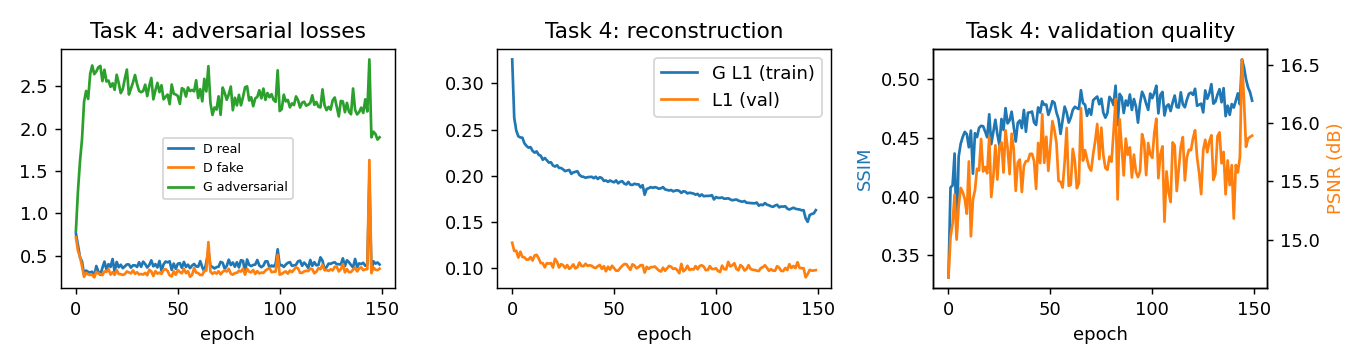
\includegraphics[width=\textwidth]{curves_task4.png}
\caption{Task 4 training: discriminator real/fake loss, generator adversarial loss, generator $L_1$ (train/val) and validation PSNR/SSIM.}
\label{fig:curves4}
\end{figure*}

\begin{figure*}[t]
\centering
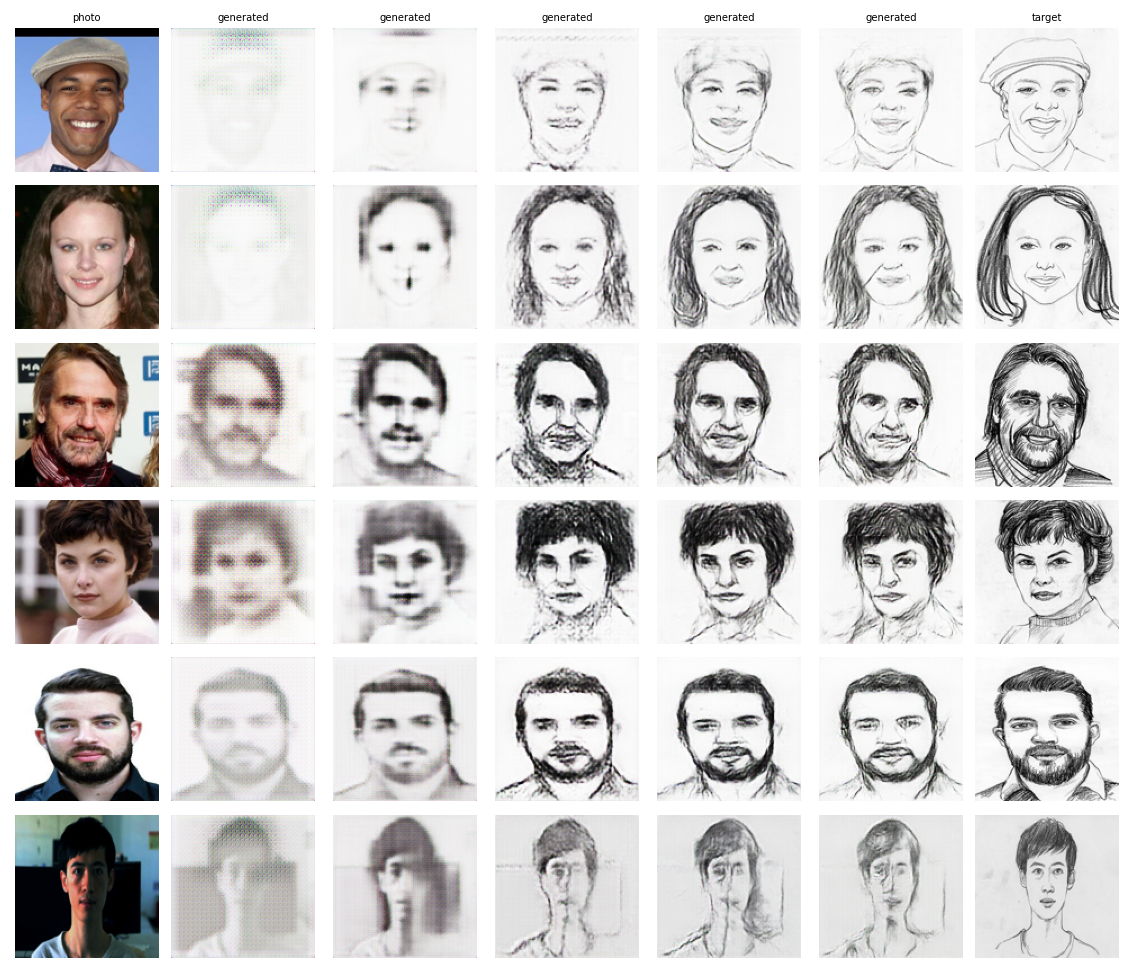
\includegraphics[width=0.85\textwidth]{t4_progress.png}
\caption{Generator development on fixed validation photographs (columns: photograph, generated sketch at epochs 1, 10, 50, 100, 150, ground-truth sketch).}
\label{fig:t4prog}
\end{figure*}

\begin{table}[t]
\centering
\caption{Task 4 test results on the official FS2K test set (images in [0,1]).}
\label{tab:t4_test}
\footnotesize
\begin{tabular}{lrrrr}
\toprule
Style & L1 & PSNR (dB) & SSIM & n \\
\midrule
all & 0.1023 & 15.91 & 0.493 & 1046 \\
Style 1 & 0.0747 & 17.84 & 0.542 & 619 \\
Style 2 & 0.1522 & 12.40 & 0.397 & 381 \\
Style 3 & 0.0611 & 19.09 & 0.629 & 46 \\
\bottomrule
\end{tabular}
\end{table}


\textbf{Results.} On the official test set the generator reaches $L_1=0.102$, 15.9\,dB and SSIM 0.493 (Table~\ref{tab:t4_test}). Performance differs by style: Style~1 (619 test pairs) 17.8\,dB / 0.542, Style~2 (381 pairs) 12.4\,dB / 0.397 and Style~3 (only 46 pairs, so a noisy estimate) 19.1\,dB / 0.629. Pixel metrics are low in absolute terms because hand-drawn strokes are not pixel-aligned with edges in the photograph, and Style~2 sketches are dark and heavily hatched, which an $L_1$-driven generator reproduces as softer, smoother strokes (Figs.~\ref{fig:t4fail}, \ref{fig:t4style}); metrics such as FID or LPIPS were not computed. The style embedding is used by both networks, and the conditioning has a clear effect (Fig.~\ref{fig:t4style}): for the same photographs, Style~1 yields light, thin contour sketches while Style~2 and Style~3 yield darker, bolder shading.

\begin{figure}[t]
\centering
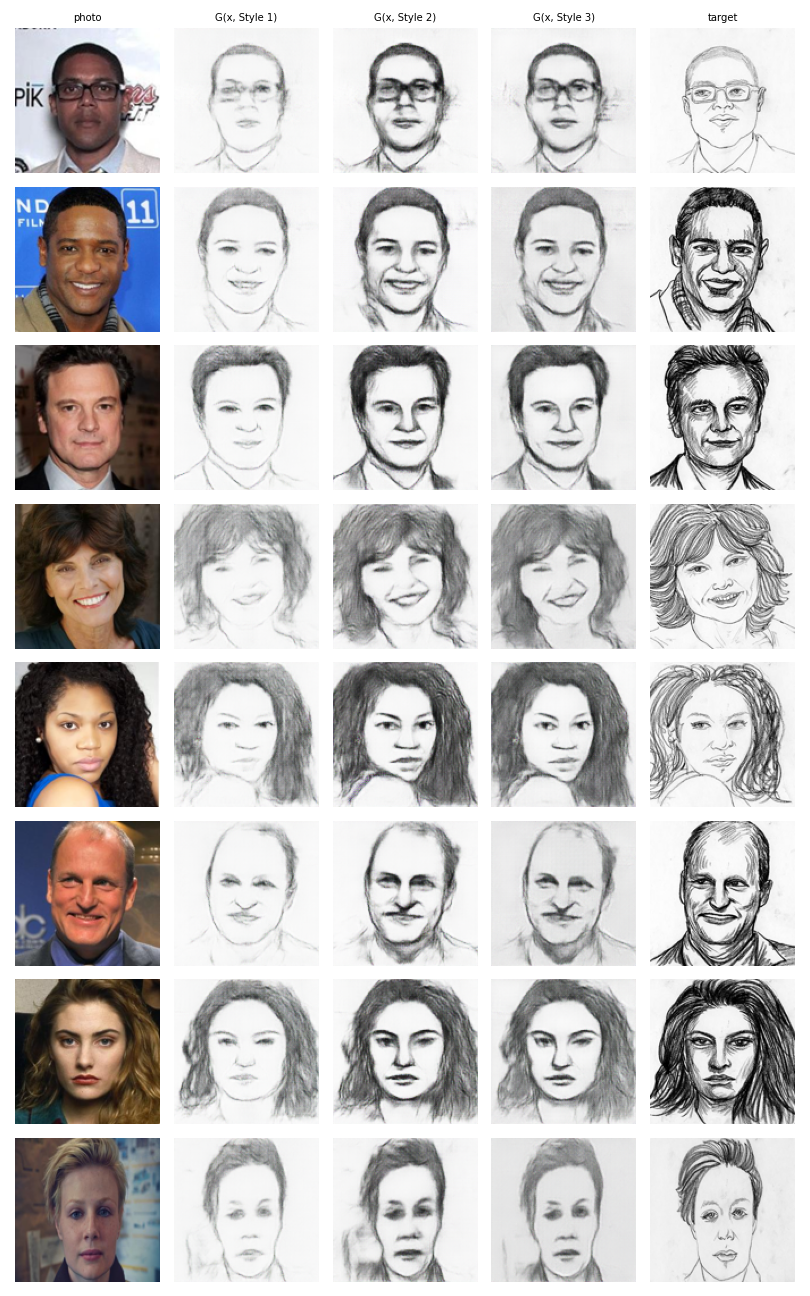
\includegraphics[width=0.9\columnwidth]{t4_style_conditioning.png}
\caption{Conditioning check on test photographs: $G(x,\text{Style 1/2/3})$ and the ground-truth sketch.}
\label{fig:t4style}
\end{figure}

\begin{figure}[t]
\centering
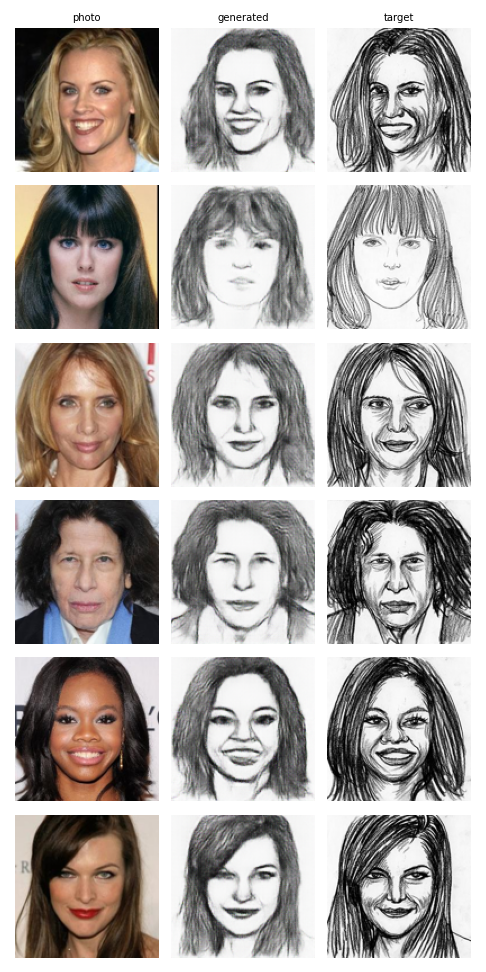
\includegraphics[width=0.6\columnwidth]{t4_failures.png}
\caption{Lowest-SSIM test examples: the generated sketches are plausible but the strokes differ from the artist's dense hatching, which pixel-wise metrics penalise heavily.}
\label{fig:t4fail}
\end{figure}

\subsection{ONNX Export and Consistency}
All seven inference models (universal autoencoder, classifier, three specialists, soft-MoE pipeline and sketch generator) were exported to ONNX (opset 17, dynamic batch) and run with ONNX Runtime on real test inputs (deterministically corrupted test images and FS2K photographs). Table~\ref{tab:onnx} shows that the maximum absolute difference to PyTorch is below $4\times10^{-6}$, far below the $10^{-4}$ threshold, for every model. On the development laptop's CPU (Intel i5-7200U) the application measured about 25\,ms per image for the universal autoencoder, about 104\,ms for the full soft-MoE pipeline and 67\,ms for the sketch generator.

\begin{table}[t]
\centering
\caption{PyTorch vs.\ ONNX Runtime consistency (max abs.\ difference, real test images).}
\label{tab:onnx}
\footnotesize
\begin{tabular}{lrcr}
\toprule
Model & max |diff| & passed ($<10^{-4}$) & size (MB) \\
\midrule
universal\_ae & 7.15e-07 & yes & 9.6 \\
classifier & 1.19e-07 & yes & 21.2 \\
specialist\_salt & 8.05e-07 & yes & 9.6 \\
specialist\_blur & 7.00e-07 & yes & 9.6 \\
specialist\_occ & 5.36e-07 & yes & 9.6 \\
soft\_moe & 4.77e-07 & yes & 50.0 \\
sketch\_generator & 3.87e-06 & yes & 168.5 \\
\bottomrule
\end{tabular}
\end{table}


\subsection{Experiment Tracking}
Every training run and every Optuna trial was logged to MLflow (parameters, per-epoch metrics, validation samples and checkpoints; the SQLite database is in \texttt{experiments/}). Fig.~\ref{fig:mlflow} shows the MLflow views of the Task~3 run table and the Task~4 metric charts. Figures of the Optuna optimisation histories (universal autoencoder, soft MoE and GAN) are in Fig.~\ref{fig:optuna}.

\begin{figure*}[t]
\centering
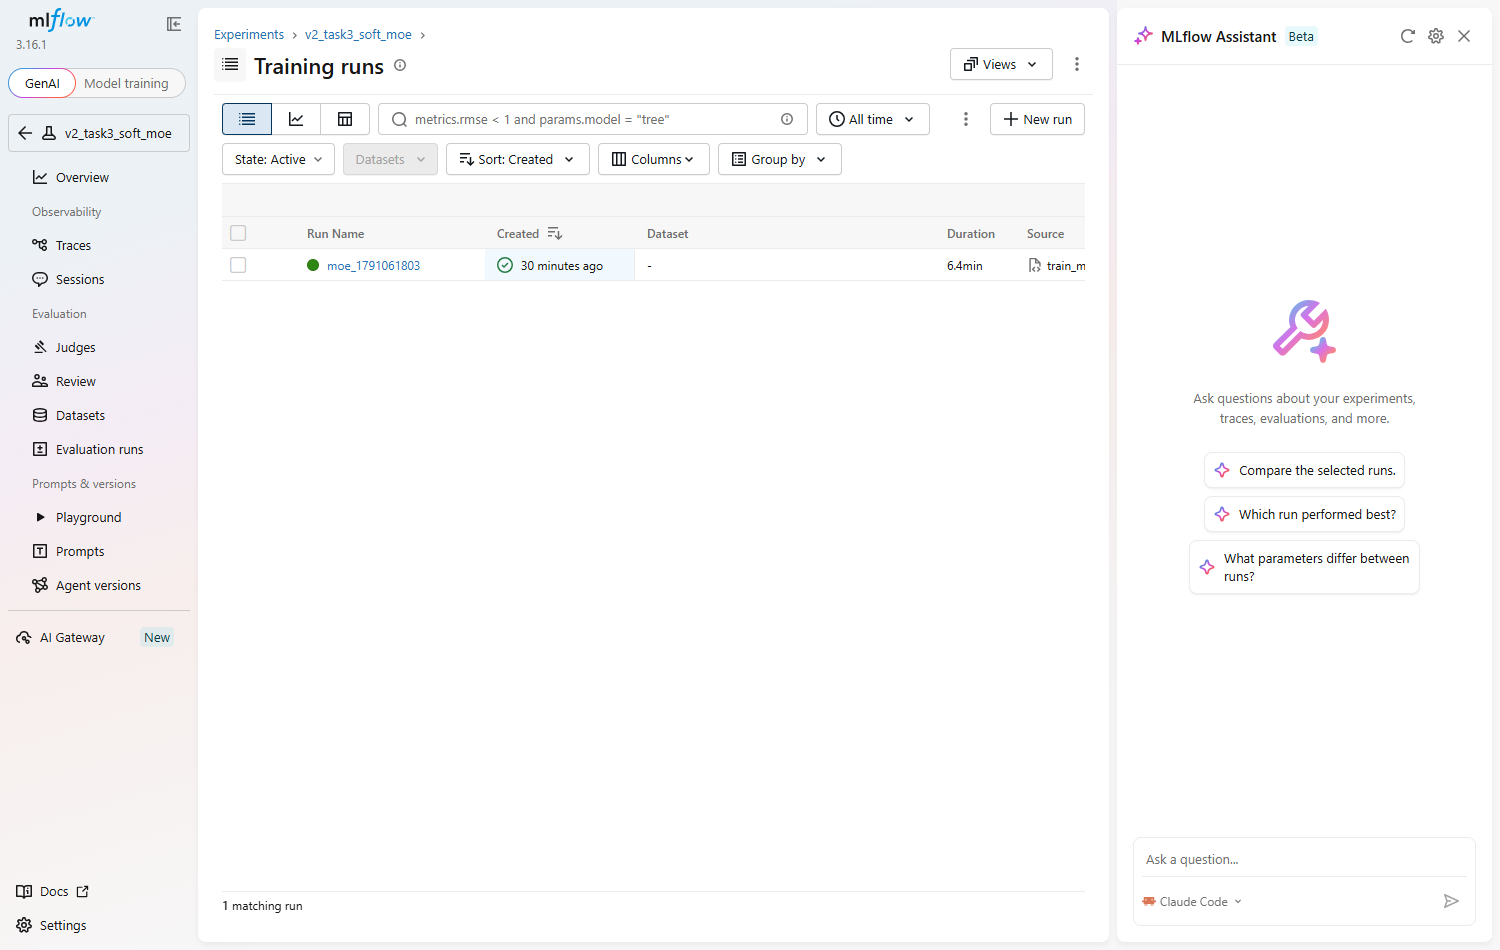
\includegraphics[width=0.48\textwidth]{mlflow_runs_task3.png}\hfill
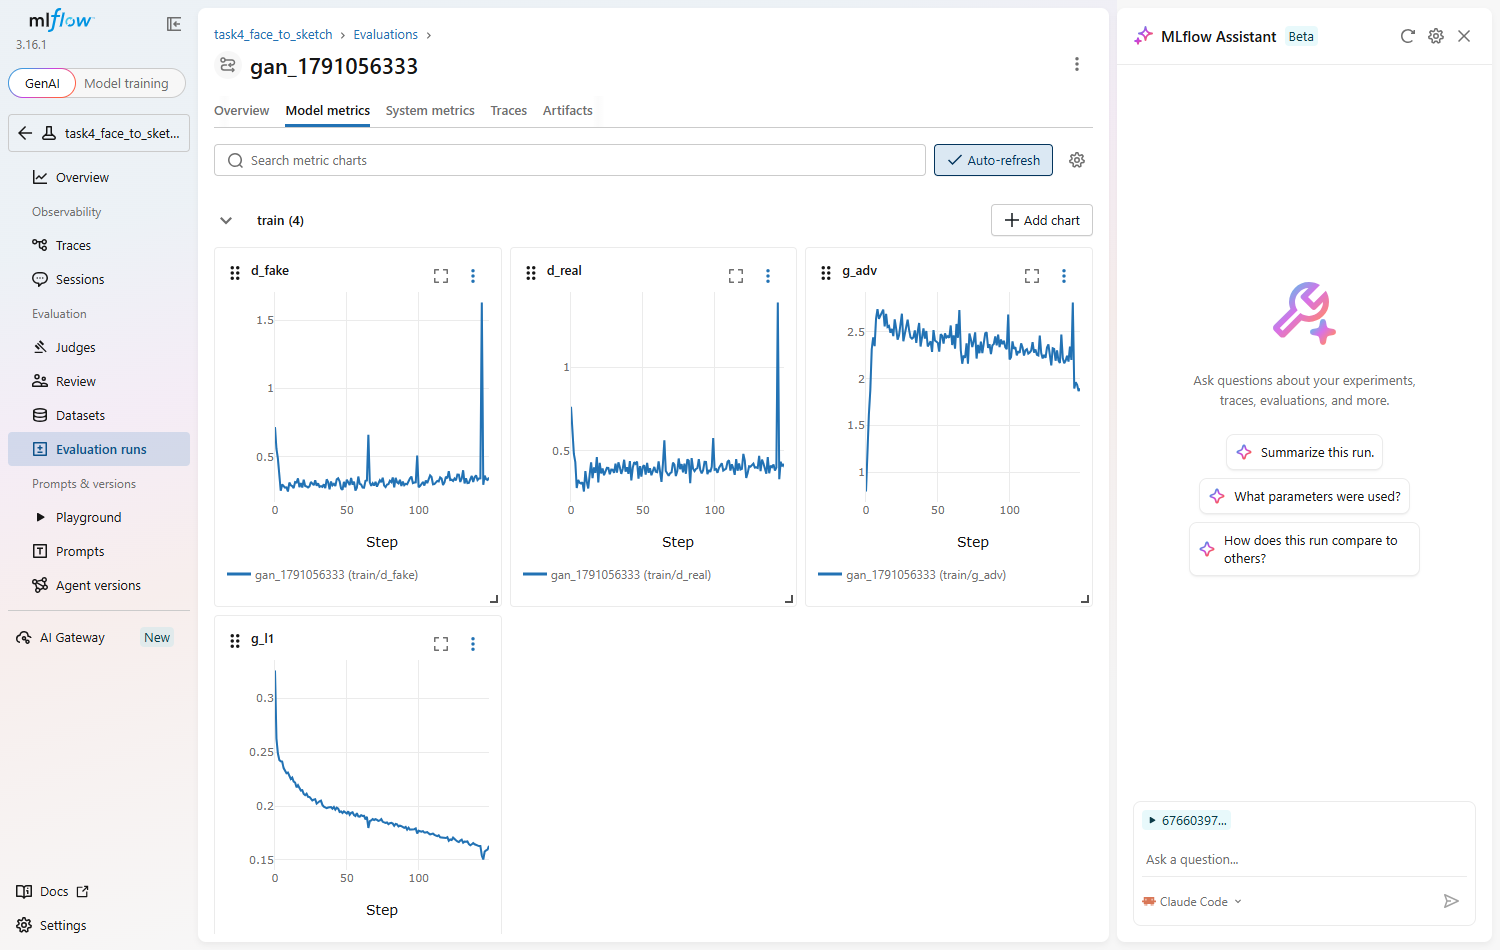
\includegraphics[width=0.48\textwidth]{mlflow_metrics_task4.png}
\caption{MLflow tracking UI: Task~3 experiment run table (left) and Task~4 training metric charts (right).}
\label{fig:mlflow}
\end{figure*}

\begin{figure*}[t]
\centering
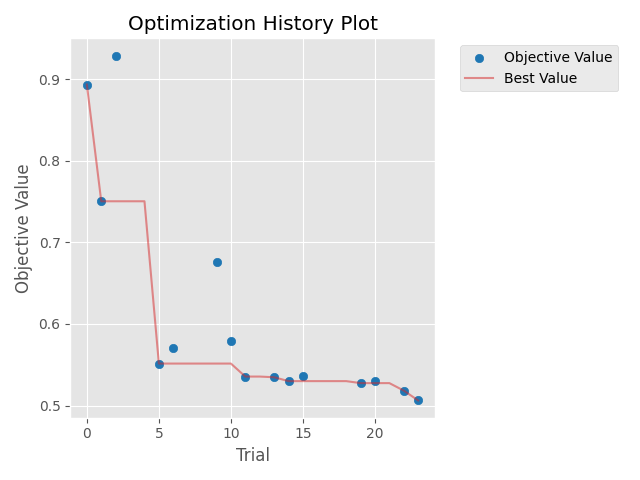
\includegraphics[width=0.32\textwidth]{optuna_universal_history.png}\hfill
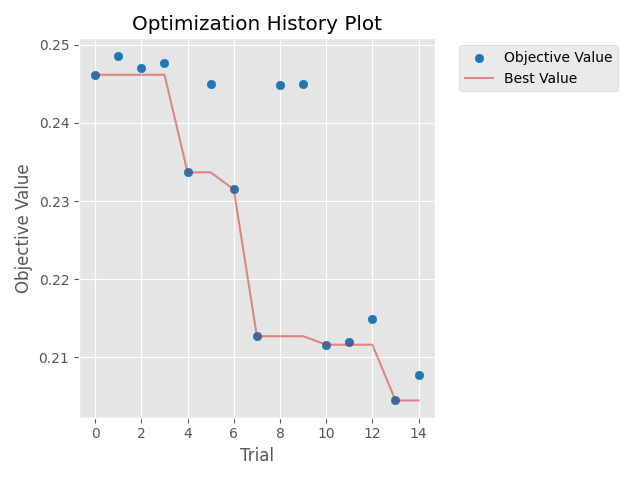
\includegraphics[width=0.32\textwidth]{optuna_moe_history.png}\hfill
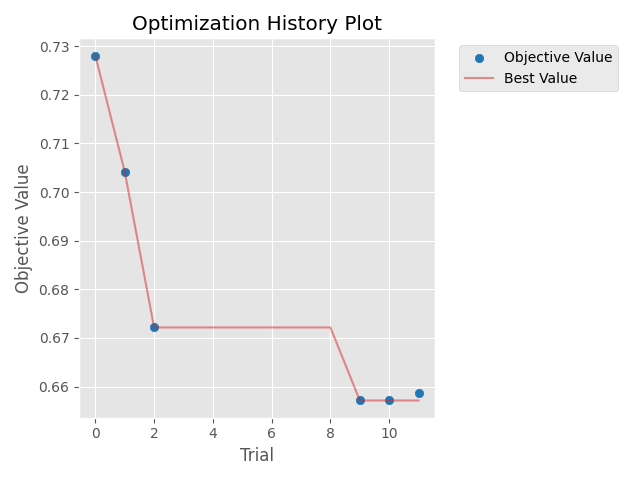
\includegraphics[width=0.32\textwidth]{optuna_gan_history.png}
\caption{Optuna optimisation histories: Task~1 universal autoencoder, Task~3 soft MoE, Task~4 cGAN.}
\label{fig:optuna}
\end{figure*}

\section{Application Screenshots}
\label{sec:appshots}
Figs.~\ref{fig:app1}--\ref{fig:app4} show the four workspaces of the running application with the final ONNX models (screenshots taken with the same Docker-independent dev stack; the Docker Compose stack serves the identical frontend and backend). The Universal and Hard-Routed pages show the clean reference, corrupted input, restored output and error map, the selected corruption settings and the inference time; the Hard-Routed page additionally shows the four classifier probabilities, the predicted corruption and the selected expert; the Soft-MoE page shows the four routing weights with the strongest contributors; the Face-to-Sketch page supports upload or webcam, the three style conditions, side-by-side display and a download button.

\begin{figure*}[t]
\centering
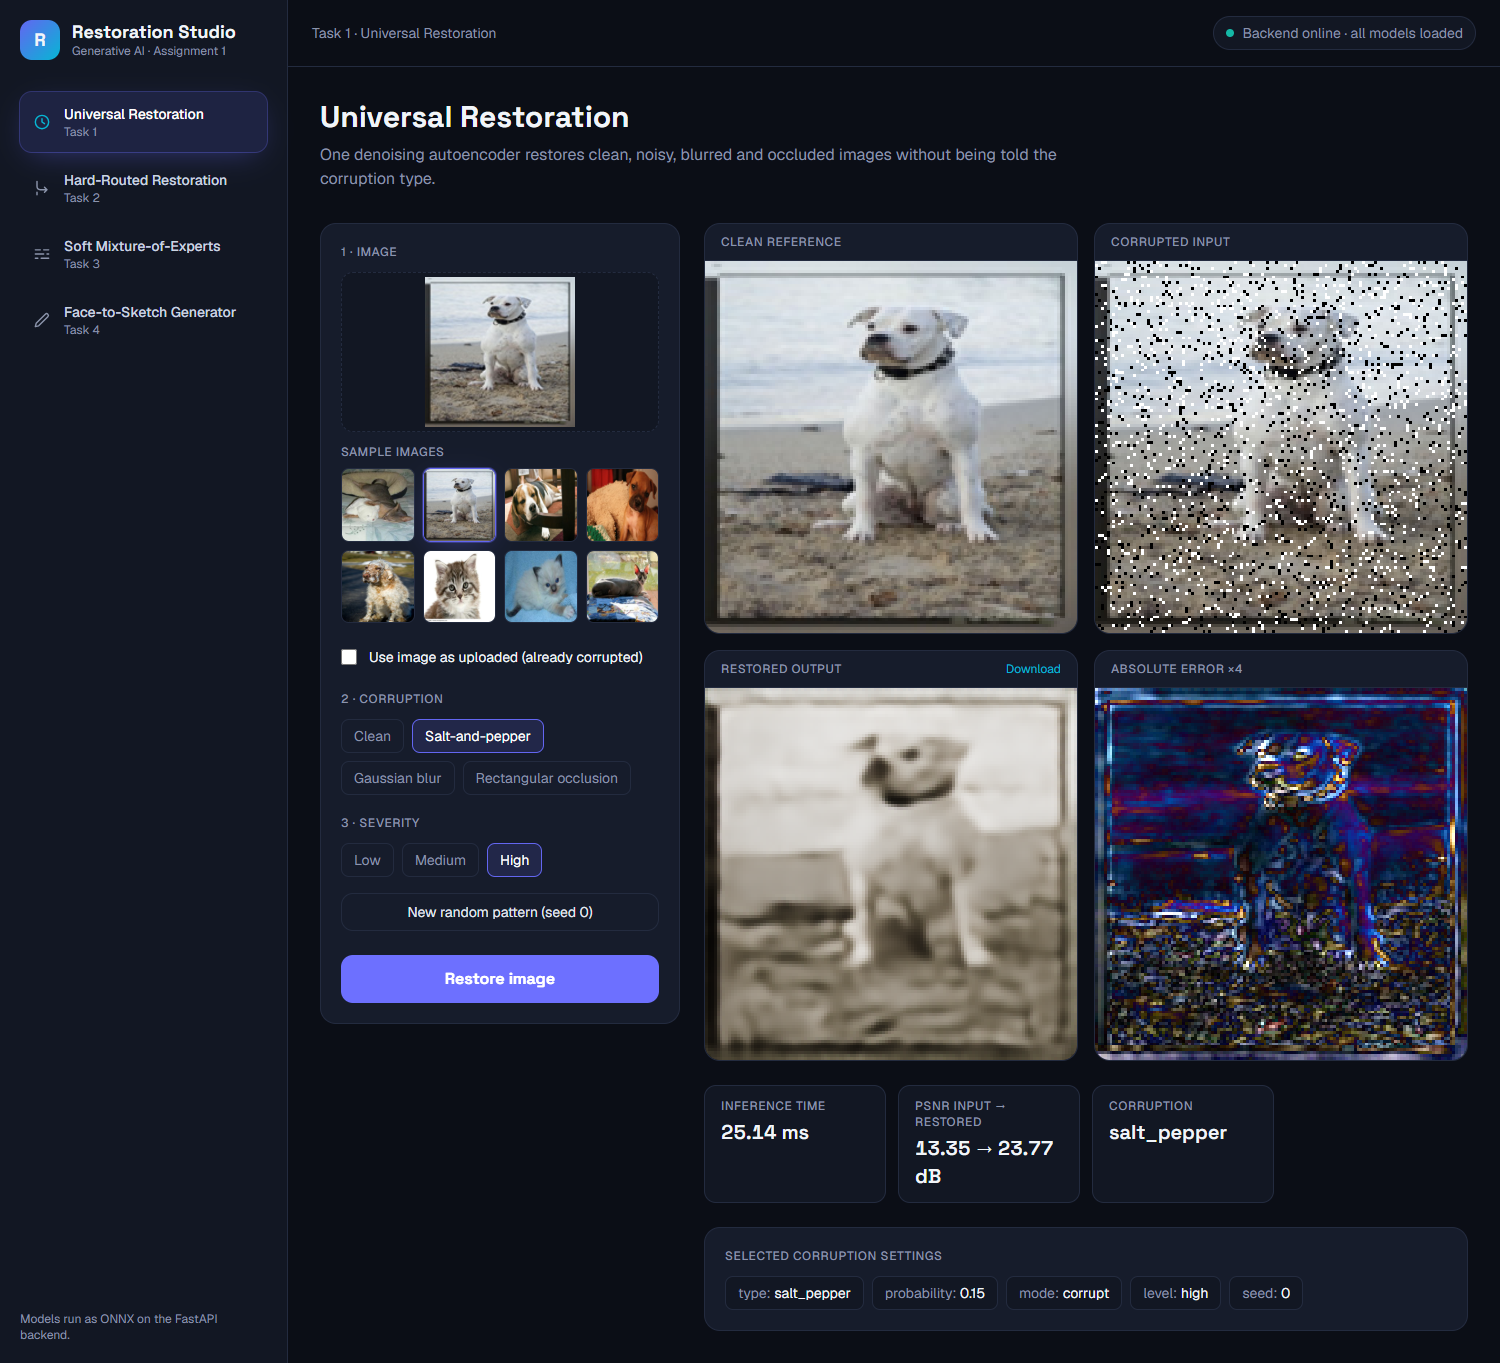
\includegraphics[width=0.72\textwidth]{app_universal.png}
\caption{Universal Restoration workspace (salt-and-pepper, high severity).}
\label{fig:app1}
\end{figure*}
\begin{figure*}[t]
\centering
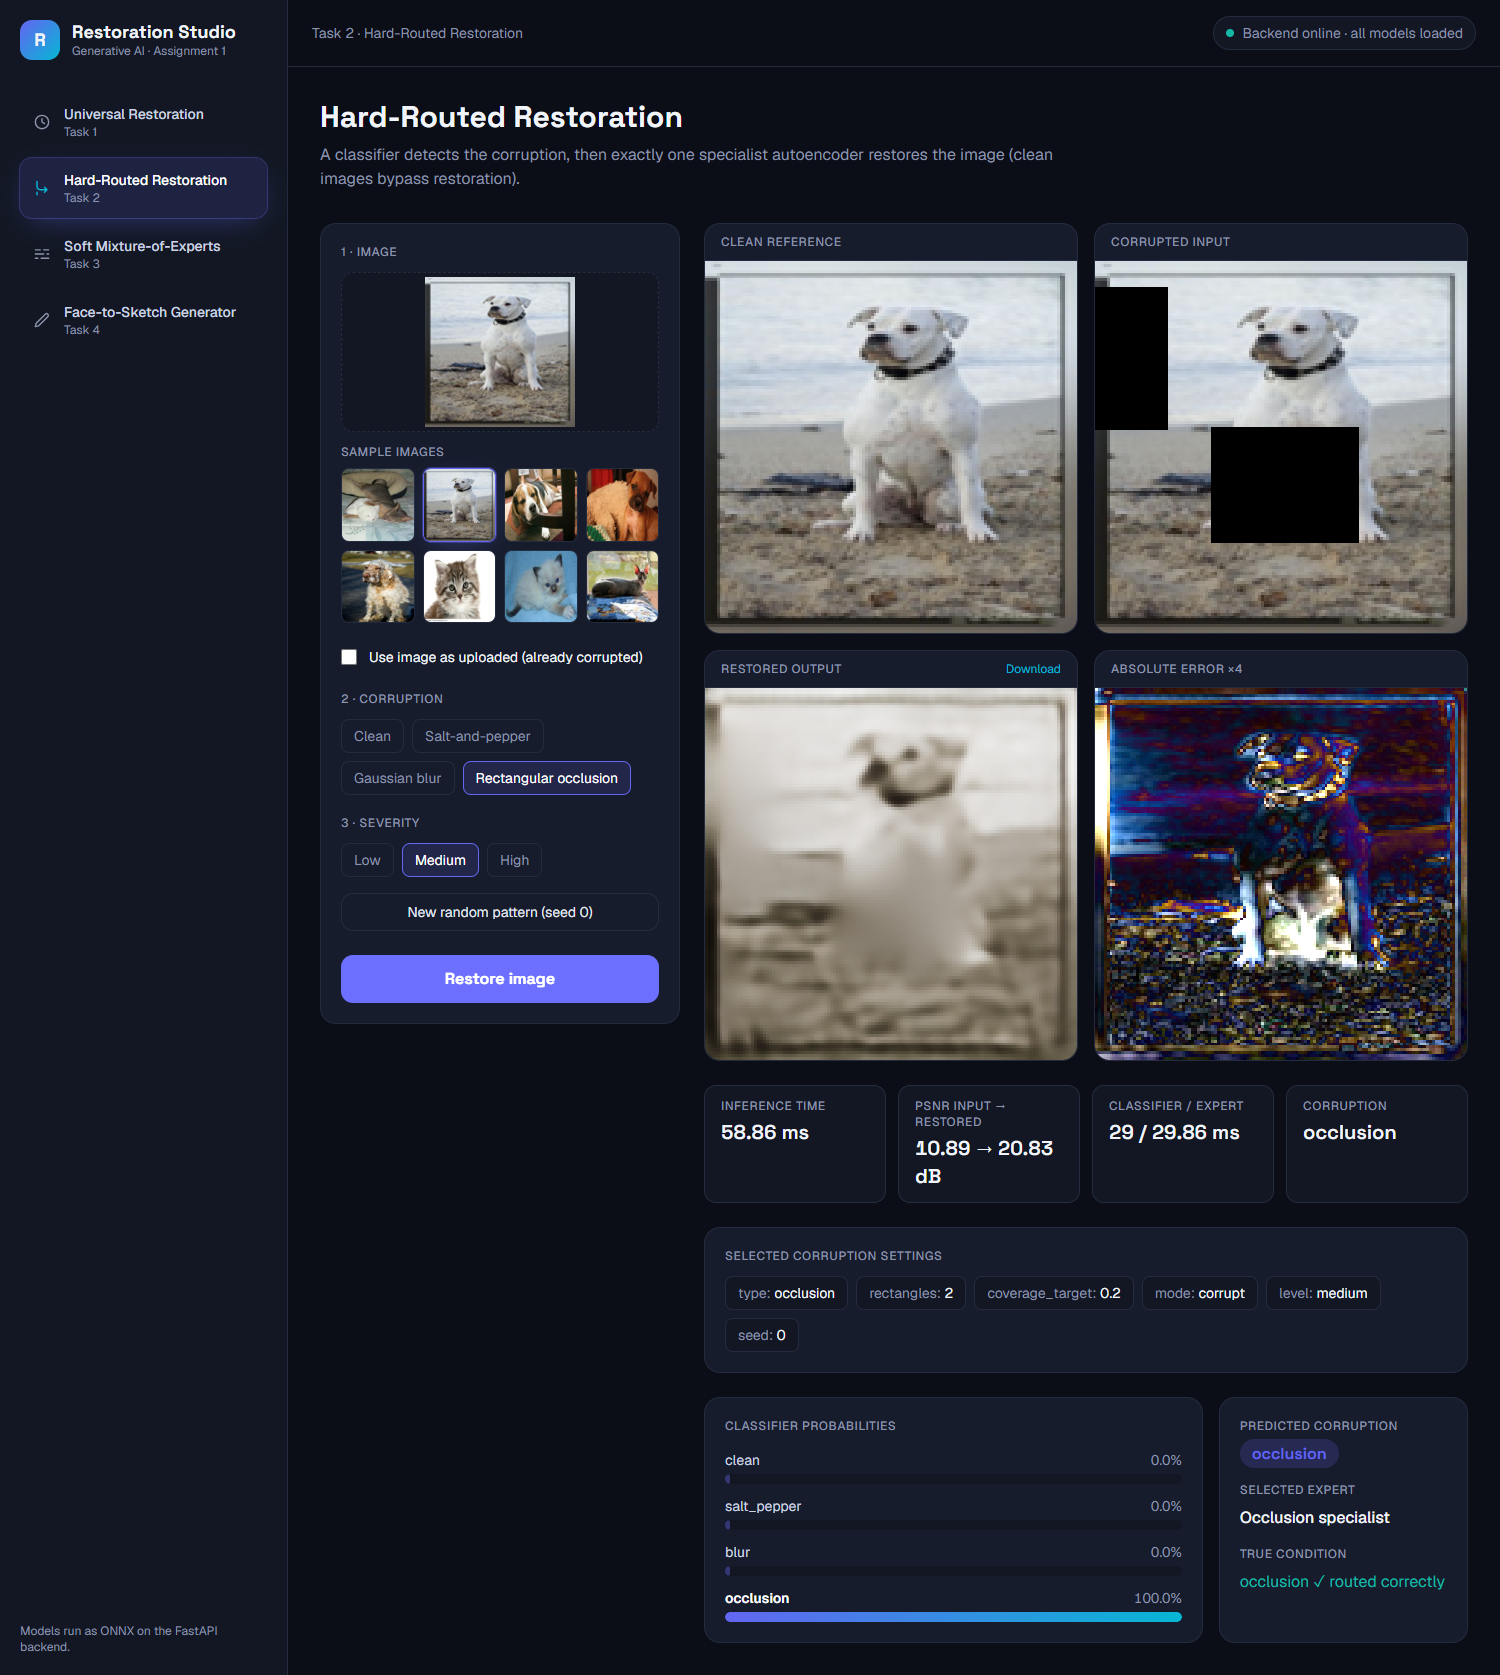
\includegraphics[width=0.72\textwidth]{app_hard_routed.png}
\caption{Hard-Routed Restoration workspace: classifier probabilities, predicted corruption and selected expert.}
\label{fig:app2}
\end{figure*}
\begin{figure*}[t]
\centering
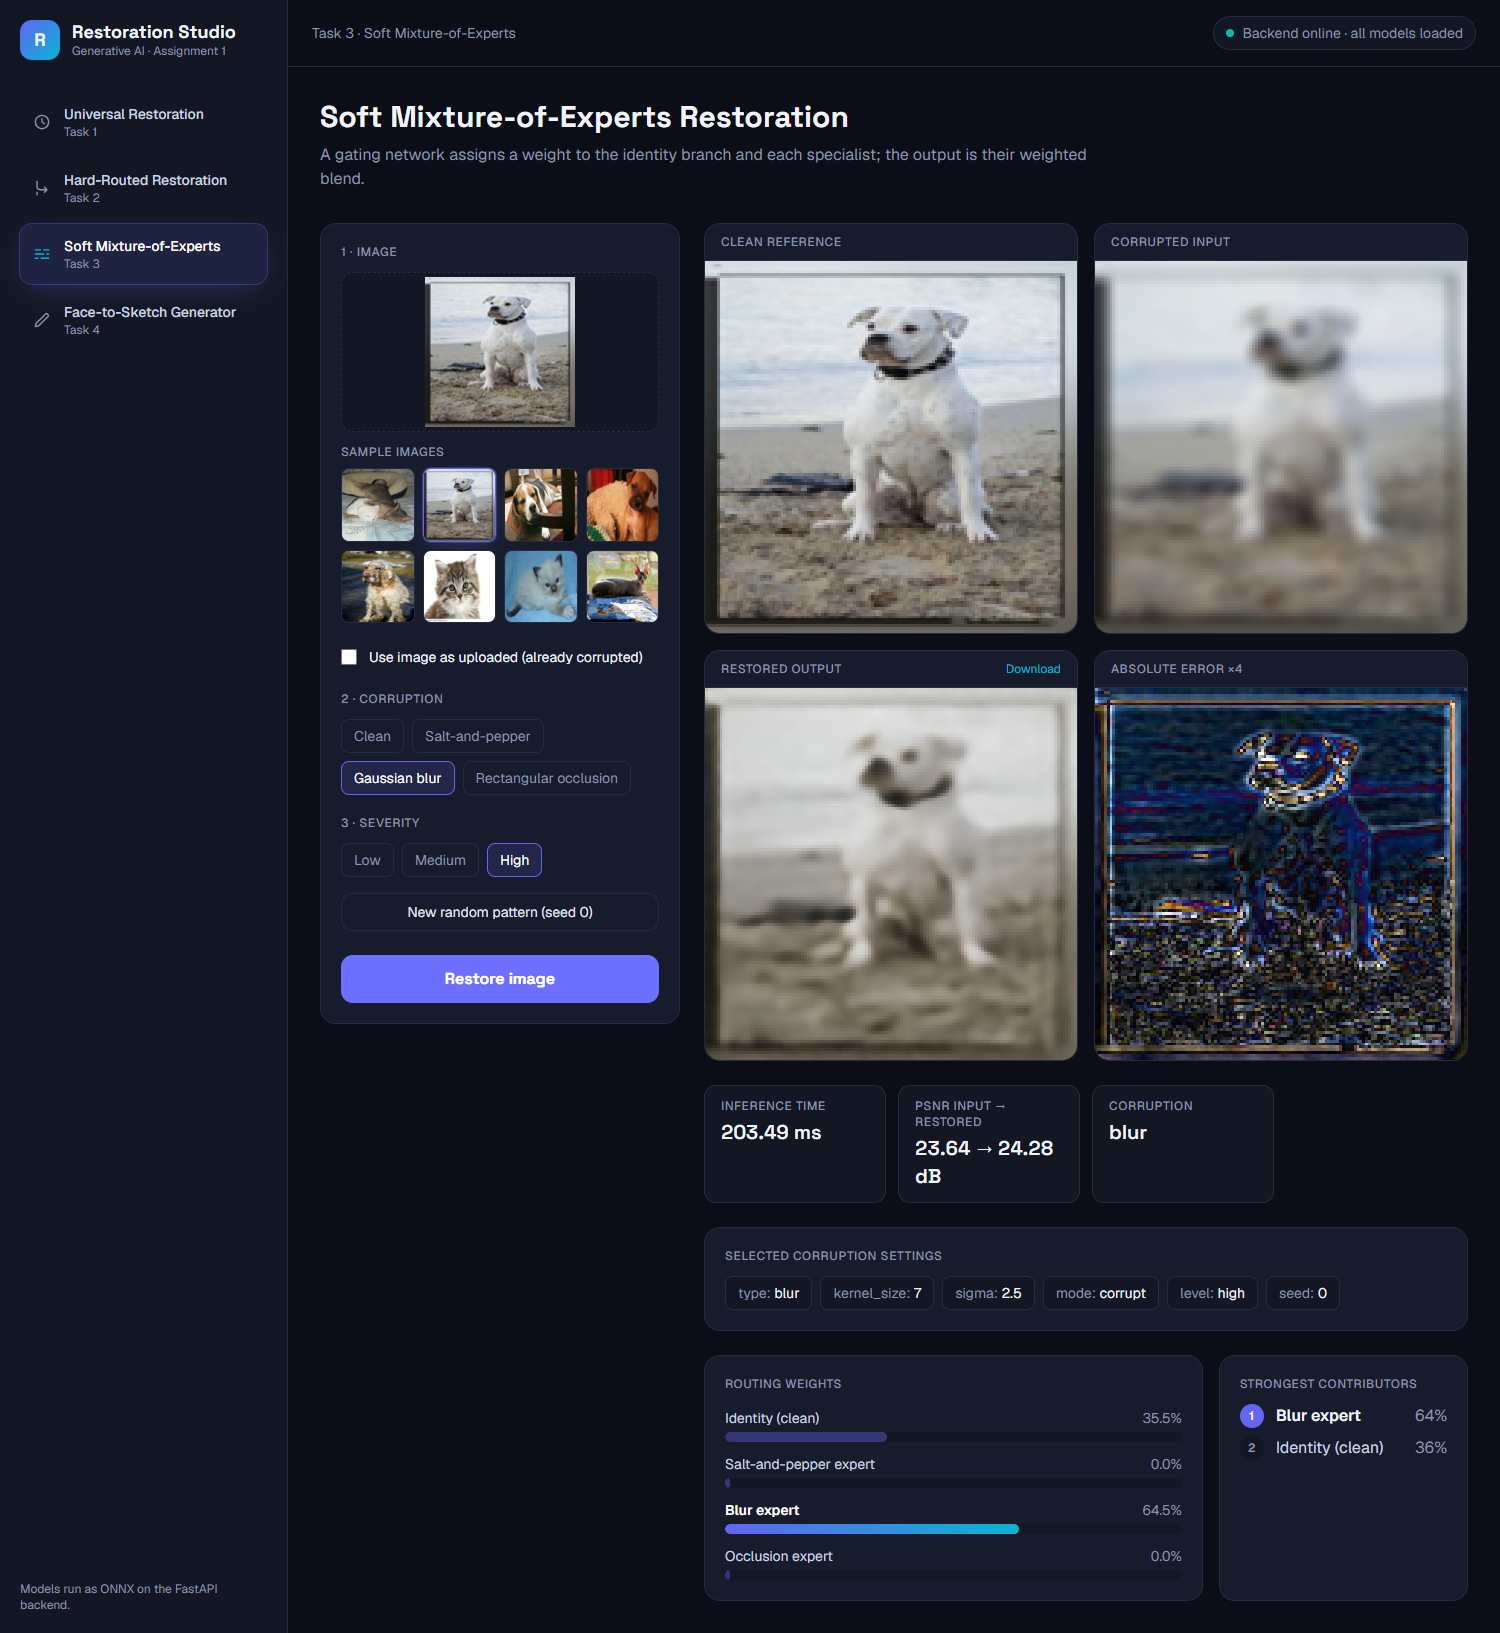
\includegraphics[width=0.72\textwidth]{app_soft_moe.png}
\caption{Soft Mixture-of-Experts workspace: routing weights and contributing experts.}
\label{fig:app3}
\end{figure*}
\begin{figure*}[t]
\centering
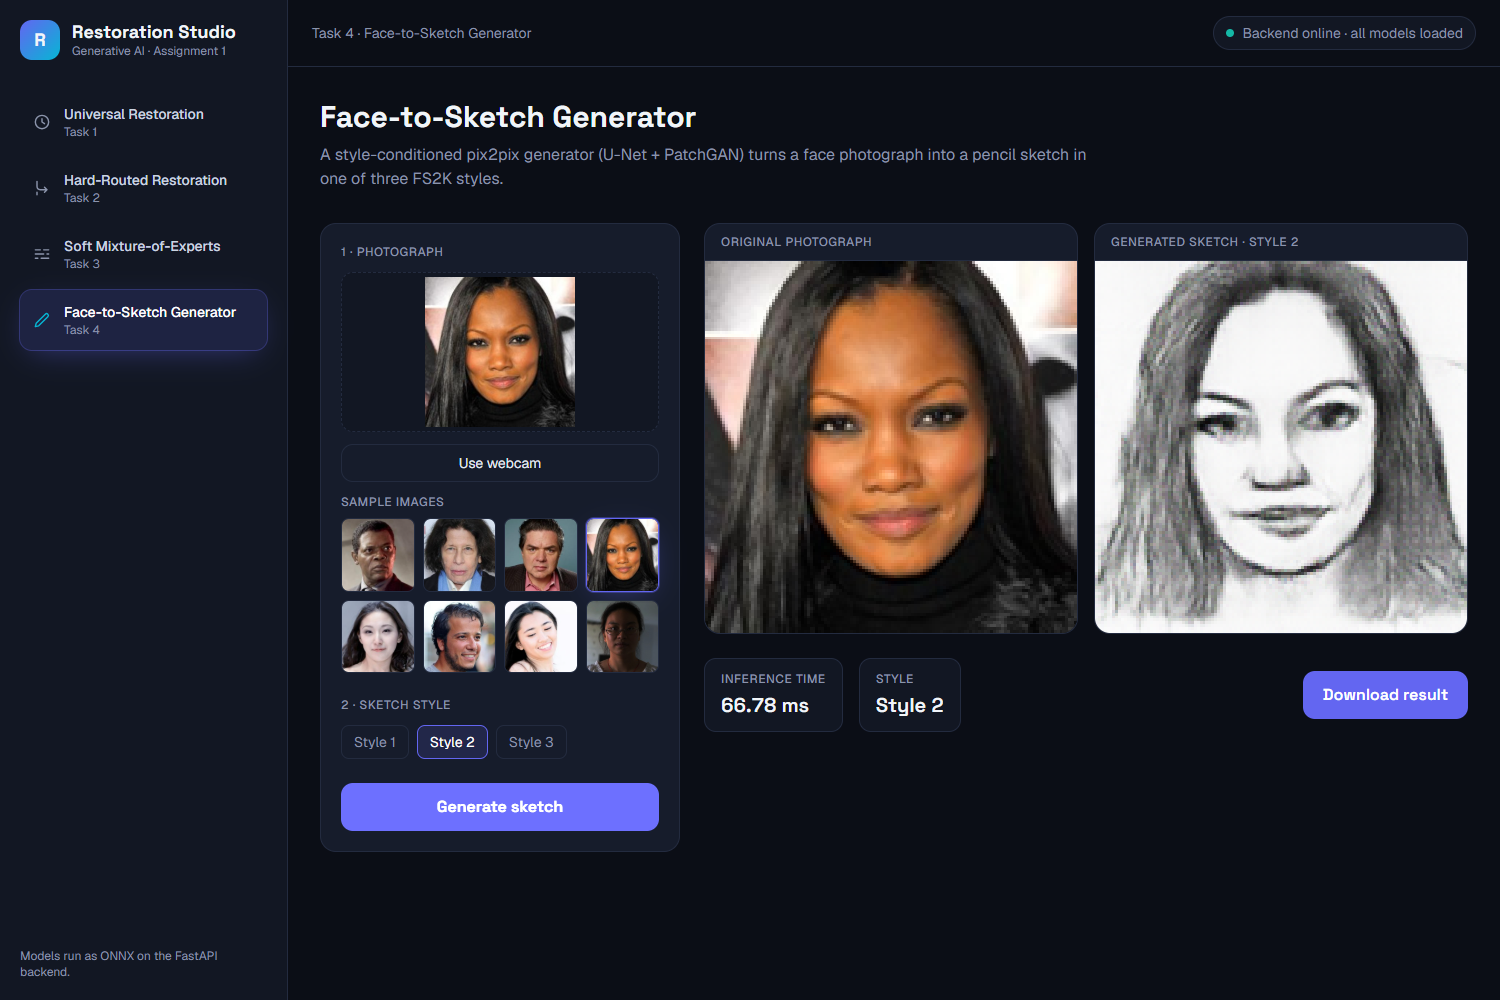
\includegraphics[width=0.72\textwidth]{app_face_to_sketch.png}
\caption{Face-to-Sketch Generator workspace (Style~2) with side-by-side result and download.}
\label{fig:app4}
\end{figure*}

\section{Limitations}
\label{sec:limits}
\begin{itemize}
\item \textbf{Reduced search budgets.} Optuna trials used 6--8 epochs on a 1{,}500-image subset (10 epochs for the GAN) and 12--24 trials per task; the CPU/GPU budget (a free Colab T4 and a one-day deadline) did not allow larger studies. $\lambda_{L1}$ for the GAN landed near the edge of its range and the autoencoder objective also favoured the largest searched latent size, so wider ranges could improve results. Each configuration was run with a single seed, so small differences (e.g.\ oracle vs.\ predicted routing, 0.001 SSIM) are not statistically established.
\item \textbf{Bottlenecked reconstruction.} With a genuine bottleneck and no skip connections the restoration autoencoders cannot match the fidelity of mildly damaged inputs (blur, low-severity noise, clean). The identity branch of Tasks~2 and 3 compensates, but the specialists remain weaker than the input in that regime; a limited skip connection (allowed by the assignment if justified) was not investigated.
\item \textbf{Soft-MoE interpretability.} The tuned classification weight is small, so the gate acts as a severity-adaptive blender rather than a classifier (argmax routing 0.673); a larger $\lambda_{CE}$ would make weights more class-like at some cost in quality (we did not tune this trade-off with a routing-aware objective). Compound corruptions (e.g.\ blur + noise) were not evaluated.
\item \textbf{GAN evaluation.} Only PSNR/SSIM/$L_1$ were used (no FID/LPIPS or user study); Style~3 has just 46 test pairs; FS2K contains few demographics; training images are only $128\times128$.
\item \textbf{Deployment.} Models run on CPU through ONNX Runtime; the demo corrupts uploaded images with the same synthetic operators as in training, so genuinely different real-world corruptions may behave differently. The Docker images were built and smoke-tested in continuous integration on GitHub; the models are supplied separately (download link in the README).
\end{itemize}

\section{Conclusion}
We built and compared three restoration strategies on a common data protocol. A universal convolutional autoencoder with a genuine latent bottleneck restores severe noise and occlusion but cannot beat mildly damaged inputs; a bottleneck that keeps spatial layout is essential (18.4$\to$21.2\,dB over a dense latent). Hard routing by a 99.6\,\%-accurate classifier with specialists and an identity bypass raises the test PSNR to 24.8\,dB with predicted routing equal to oracle routing, but its rare errors on clean images are destructive. A jointly fine-tuned soft MoE reaches 26.3\,dB / 0.814 SSIM by blending identity and experts according to severity, at the price of gate weights that no longer mirror the corruption label. A style-conditioned pix2pix generator with a learned style embedding produces recognisable, style-dependent sketches (test SSIM 0.49), and all four systems were tuned with Optuna, tracked with MLflow, verified against ONNX and deployed in a single web application whose Docker Compose configuration starts the complete stack.

\appendices
\section{AI-Use Statement}
The following AI tools were used. \emph{Anthropic's Claude} (a large-language-model coding assistant) helped with drafting and debugging code (data pipeline, training and evaluation scripts, backend, frontend, Docker configuration) and with editing the documentation and this report. \emph{Google Stitch} was used to produce the first interface design (Fig.~\ref{fig:stitch}). The author chose the research directions and design decisions, directed the experiments, reviewed the results, and is responsible for the submitted work. AI output was tested and corrected rather than trusted: unit tests for the data pipeline, corruptions, metrics, models and API; a numerical comparison of the PyTorch and ONNX outputs; a continuous-integration build of the Docker stack; and end-to-end runs of the application on the trained models. Bugs found this way (for example a half-precision type mismatch in the hard router and upper-case file extensions that fail on Linux) were fixed, and all numerical results reported here are copied by script from the files produced by the final runs. The author can explain and modify any component.

\section{Reproduction}
\textbf{Repository:} \url{https://github.com/MusaxKhan/Restoration-GAN}. The README gives the Docker commands (\texttt{python scripts/download\_models.py}, then \texttt{docker compose up --build}), the data-preparation, training, Optuna, evaluation and ONNX-export commands (\texttt{notebooks/colab\_training.ipynb}, \texttt{scripts/run\_v2.sh}, \texttt{scripts/finish\_v2.sh}), and the model download link. Experiment records (MLflow database, Optuna studies, best configurations) are under \texttt{experiments/} and \texttt{configs/}.


\bibliographystyle{IEEEtran}
\bibliography{references}

\end{document}
